
\chapter{变化检测任务基础范式设计}

\section{引言}
遥感影像变化检测旨在通过比较不同时间获取的同一地理区域影像,自动识别地表变化区域。该任务在土地利用监测、城市扩张分析、生态保护和灾害评估等应用中具有重要意义~\cite{ting_bai_deep_2023}。在计算机视觉领域,变化检测和图像分割均被视为像素级预测任务~\cite{YGXB202309001}。几乎所有像素级任务的算法都采用编码器–解码器架构,其中编码器将输入数据转化为高维特征,解码器则将这些特征重构为特定任务所需的形式。然而,变化检测任务的独特之处在于其对双时相影像的处理,通常需要使用Siamese编码器设计~\cite{dong_efficientcd_2024}。因此,目前大多数变化检测算法均基于深度学习架构~\cite{chen_remote_2022, zhang_swinsunet_2022, wang2022unetformer}。

% % (可选)在导言区统一设置最大高度
% \usepackage{graphicx}
% \setkeys{Gin}{height=0.30\textheight, keepaspectratio}

%—— 图 a ——
\begin{figure}[!htbp]
  \centering
  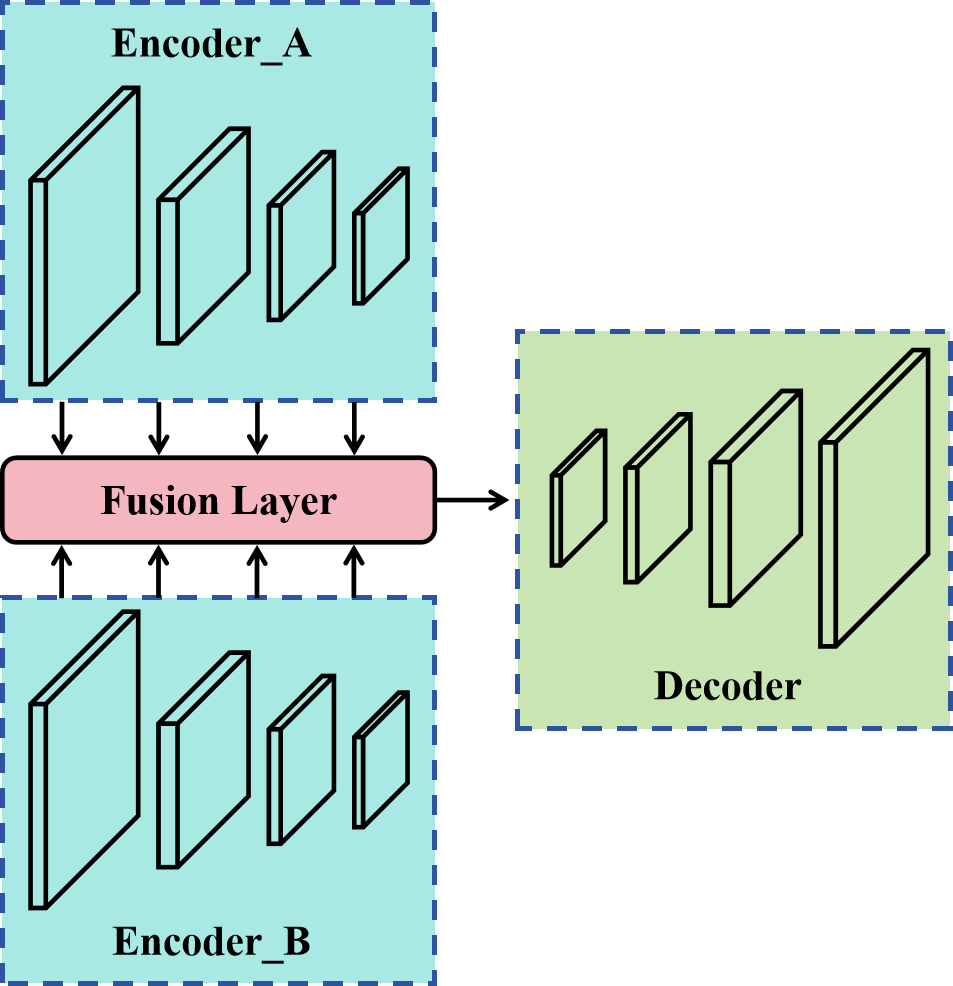
\includegraphics[width=0.6\textwidth]{paper_figures/变化检测任务基础范式设计/SEED1a.png}
  \caption{Siamese 编码器 + 融合 + 解码器。首先,Siamese 编码器提取双时相特征图,然后将这些特征图进行融合,最后对融合后的特征图进行解码。}
  \label{fig:SEED1a}
\end{figure}

%—— 图 b ——
\begin{figure}[!htbp]
  \centering
  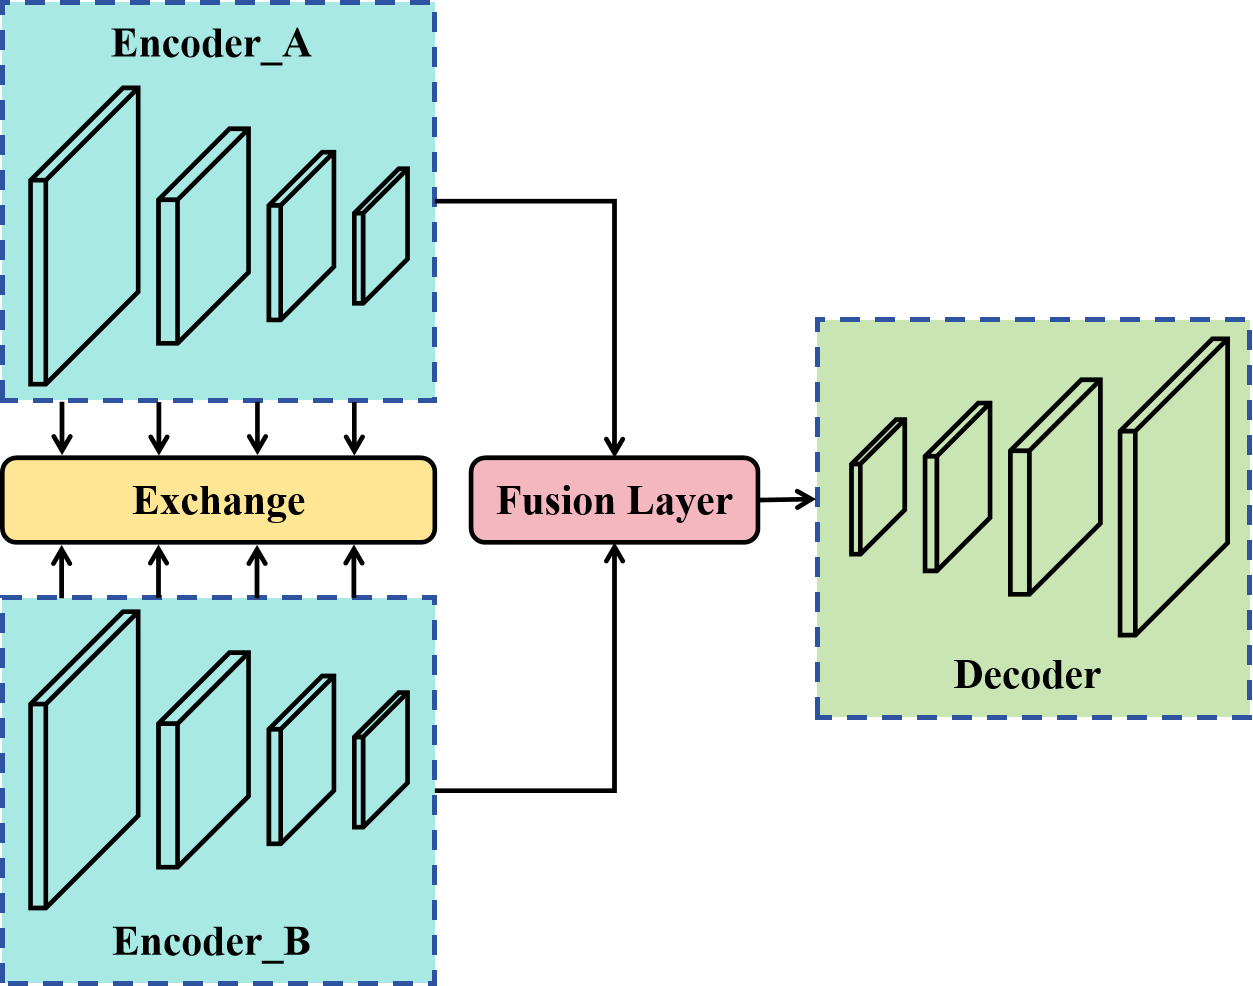
\includegraphics[width=0.6\textwidth]{paper_figures/变化检测任务基础范式设计/SEED1b.png}
  \caption{Siamese 交换(编码器)+ 融合 + 解码器。首先,Siamese 编码器在提取双时相特征图的同时进行特征交换,以增强跨时相的信息交互。交换后的特征图随后进行融合,融合后的特征图最终被解码。}
  \label{fig:SEED1b}
\end{figure}

%—— 图 c ——
\begin{figure}[!htbp]
  \centering
  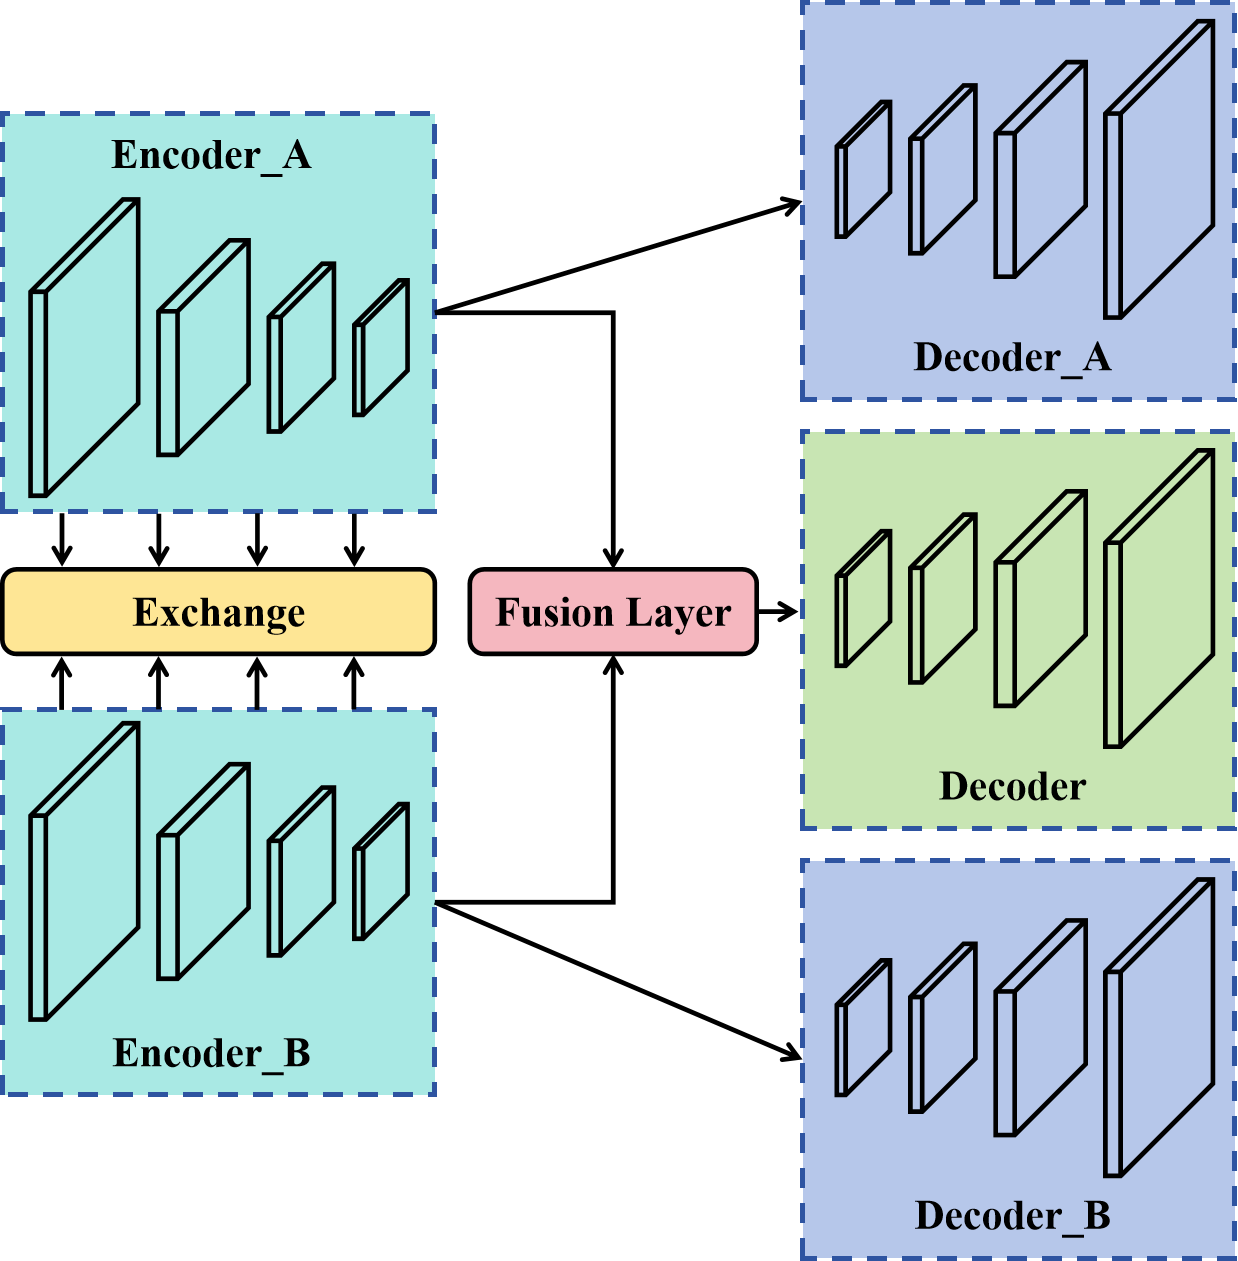
\includegraphics[width=0.6\textwidth]{paper_figures/变化检测任务基础范式设计/SEED1c.png}
  \caption{Siamese 交换(编码器)+ 融合 + 三分支解码器。首先,Siamese 编码器提取双时相特征图,同时进行特征交换,以增强跨时相的信息交互。接下来,交换后的特征图被融合并解码;此外,经过特征交换的 Siamese 编码器分支也被解码。}
  \label{fig:SEED1c}
\end{figure}

%—— 图 d ——
\begin{figure}[!htbp]
  \centering
  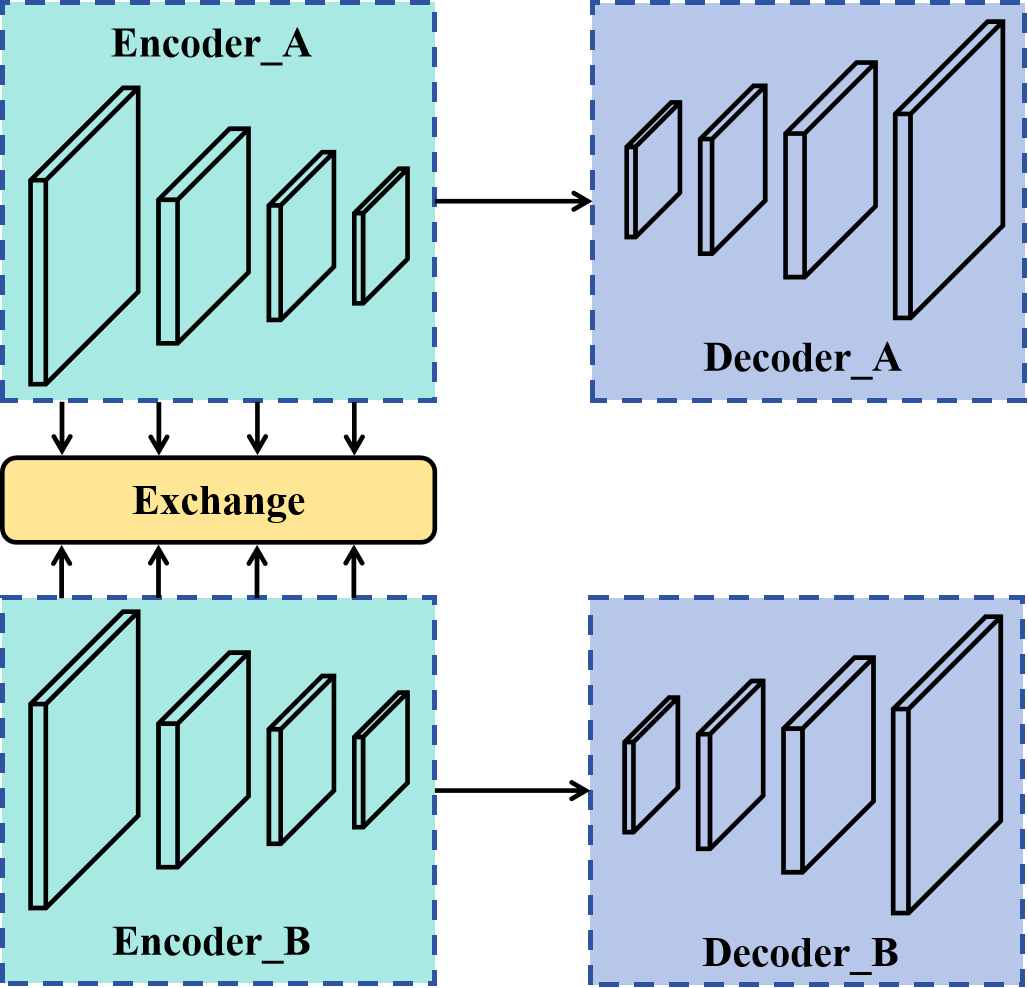
\includegraphics[width=0.6\textwidth]{paper_figures/变化检测任务基础范式设计/SEED1d.png}
  \caption{\textbf{Siamese Encoder-Exchange-Decoder (SEED)}. 首先,Siamese 编码器提取双时相特征图。这些特征图随后被交换,最后对交换后的编码器分支进行解码。}
  \label{fig:SEED1d}
\end{figure}

基于深度学习的变化检测任务的理论基础是,首先利用深度神经网络对双时相影像进行特征提取,然后设计合适的模块来学习差异特征,这些差异特征反映了双时相影像之间的差异~\cite{shi_change_2020,lv_land_2022}。基于这些差异特征,单一解码器能够逐步引导模型识别发生变化的区域。Siamese 神经网络的出现为变化检测任务的特征提取提供了尤为有效的框架~\cite{shi_deeply_2022}。在大多数常用的变化检测模型中,都构建了一个权重共享的特征提取架构。通过该 Siamese 编码器结构,模型可以从双时相影像中提取图像特征,并进一步基于这些双时相特征构建差异特征,以解码变化区域~\cite{zhu_land-useland-cover_2022-1}。


\begin{figure}[!htbp]
  \centering
  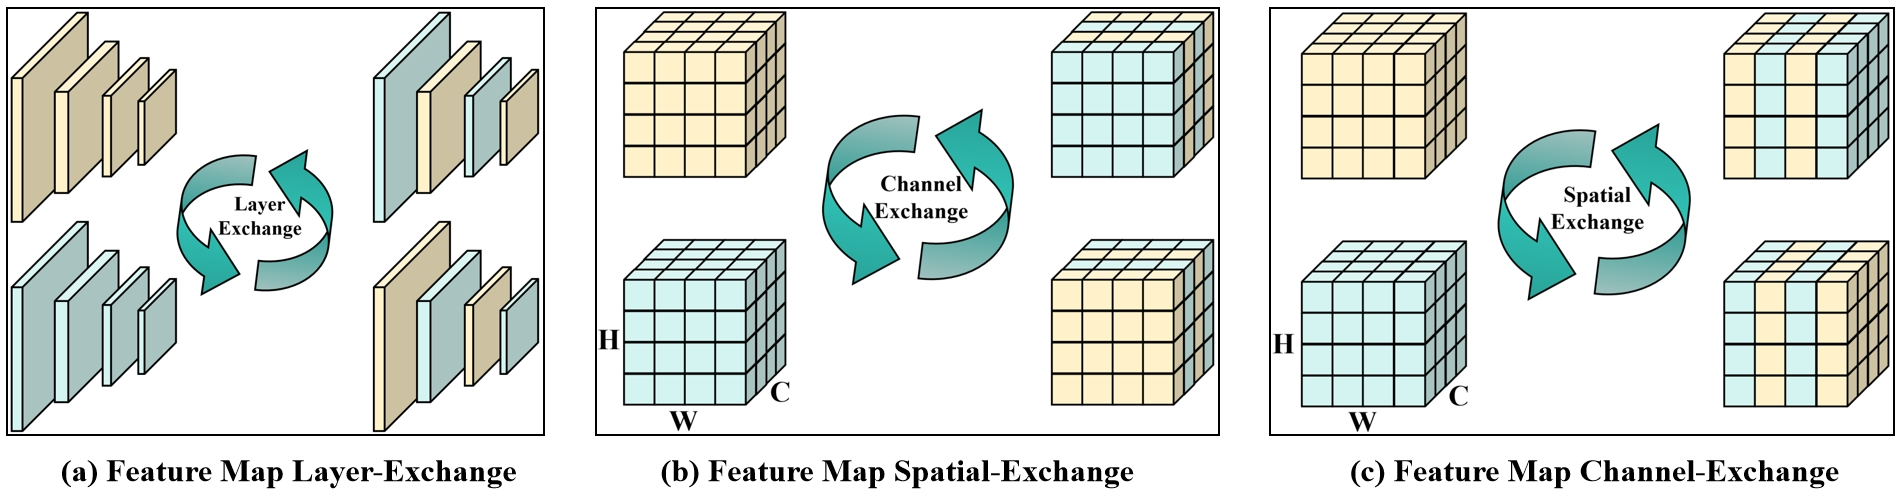
\includegraphics[width=\textwidth]{paper_figures/变化检测任务基础范式设计/seed_exchange.png}
  \caption{三种常见的特征交换方法:层交换、通道交换和空间交换。}
  \label{fig:seed_exchange}
\end{figure}

另一项广泛研究的变化检测内容是差异特征的计算~\cite{pei_feature_2022,x_zhang_difunet_2022,gu2023fdff}。由于变化检测模型以两幅影像作为输入但仅产生单一输出,因此必须在模型内部融合这两幅影像的特征。在常见的变化检测模型中,有三种简单的双时相特征融合方法(Fusion Layer):拼接(concatenation)~\cite{gu2023fdff,wan_d-tnet_2022-3,wang_hmcnet_2022-2}、逐元素相加(element-wise addition)~\cite{pei_feature_2022,gu2023fdff} 和逐元素相减(element-wise subtraction)~\cite{gu2023fdff,shi_deeply_2022,x_zhang_difunet_2022}。拼接方法将双时相特征图在通道维度上堆叠,使模型能够从堆叠后的特征图中学习变化特征;相加方法是一种深度学习中常见的特征融合技术,将两幅特征图逐元素相加,使模型能够从组合特征中提取变化信息;而相减方法则直接计算逐元素差异,以表示变化特征。

然而,利用这类数学运算构建差异特征存在一个根本性问题:这些方法在一定程度上会破坏双时相影像的原始特征。例如,通过相加或相减得到的特征与原始影像特征差异较大,可能会给模型的学习过程带来困难。

为此,研究者们提出了基于特征交换的差异学习方法,并引入了多种以特征交换为核心的范式,如图~\ref{fig:SEED1a}、~\ref{fig:SEED1b}、~\ref{fig:SEED1c}和~\ref{fig:SEED1d}所示。其中,图~\ref{fig:SEED1a} 描绘了经典的基于 Siamese 神经网络的变化检测范式,目前大多数主流变化检测算法即基于此设计;图~\ref{fig:SEED1b} 展示了一个在编码阶段通过特征交换增强双时相影像信息流的特征交换型变化检测框架;图~\ref{fig:SEED1c} 与图~\ref{fig:SEED1b} 类似,只是在解码阶段对交换后的双时相特征图分别进行解码,构建了三分支解码器。从图~\ref{fig:SEED1a}、图~\ref{fig:SEED1b} 和图~\ref{fig:SEED1c} 可以看出,目前的变化检测模型依然依赖 Fusion Layer 来合并双时相特征——因为传统框架普遍认为只有融合双时相特征才能表示变化特征。然而,本章提出了一个新颖的 Siamese Encoder-Exchange-Decoder(SEED)框架。如图~\ref{fig:SEED1d} 所示,SEED 完全摒弃了任何 Fusion Layer,仅依靠特征交换操作。与其他变化检测范式相比,SEED 显得极为简洁。

至于特征交换方法,已有研究者提出了多种基于特征交换的差异方法来改进变化检测模型,主要包括层交换~\cite{dong_efficientcd_2024}、通道交换~\cite{Fang2022ChangerFI,zhao_exchanging_2023} 以及空间交换~\cite{Fang2022ChangerFI,zhao_exchanging_2023},如图~\ref{fig:seed_exchange} 所示。这些方法利用上述三种特征交换技术来加强双时相影像之间的信息交流,从而优化变化检测模型的性能。然而,它们仍然依赖构建差异特征来学习变化区域,尚缺乏对特征交换核心原理的深入分析。

基于前人研究~\cite{dong_efficientcd_2024,Fang2022ChangerFI,zhao_exchanging_2023},可以看出变化检测的核心因素在于:只要保持双时相影像像素对应关系不变,变化检测模型的核心目标就始终是判断每个对应像素在目标类别上是否发生了变化。本章将这一原则称为“像素一致性原则”。基于此洞见,提出了一个简洁的变化检测框架——Siamese Encoder-Exchange-Decoder(SEED)框架。在 SEED 中,完全不计算差异特征,从而在整个模型中保留影像的原始信息。框架仅通过特征交换操作,使模型能在 Siamese 编码器-解码器分支中分别学习变化区域的特征。

在 SEED 框架中,Siamese 编码器共享同一组编码参数,特征交换模块不引入额外参数,Siamese 解码器也共享同一组解码参数。从本质上讲,基于 SEED 框架的变化检测架构仅需一套编码器-解码器参数,在一定程度上将变化检测任务与语义分割任务进行了统一。因此,几乎所有基于编码器-解码器结构的语义分割模型均可直接转化为基于 SEED 框架的变化检测模型。本章的主要贡献可归纳如下:

1. 提出了一种基于特征交换的全新变化检测范式——仅依赖 Siamese 编码器-解码器框架,无需计算任何差异特征,即可识别变化区域。
2. 对特征交换机制进行了深入分析,并通过大量实验验证其可解释性,提出了变化检测任务中的像素一致性原则。
3. SEED 框架实现了变化检测任务与语义分割任务的统一。设计实验证明了,可利用特征交换方法将语义分割模型高效转换为变化检测模型。


\begin{figure}[!htbp]
  \centering
  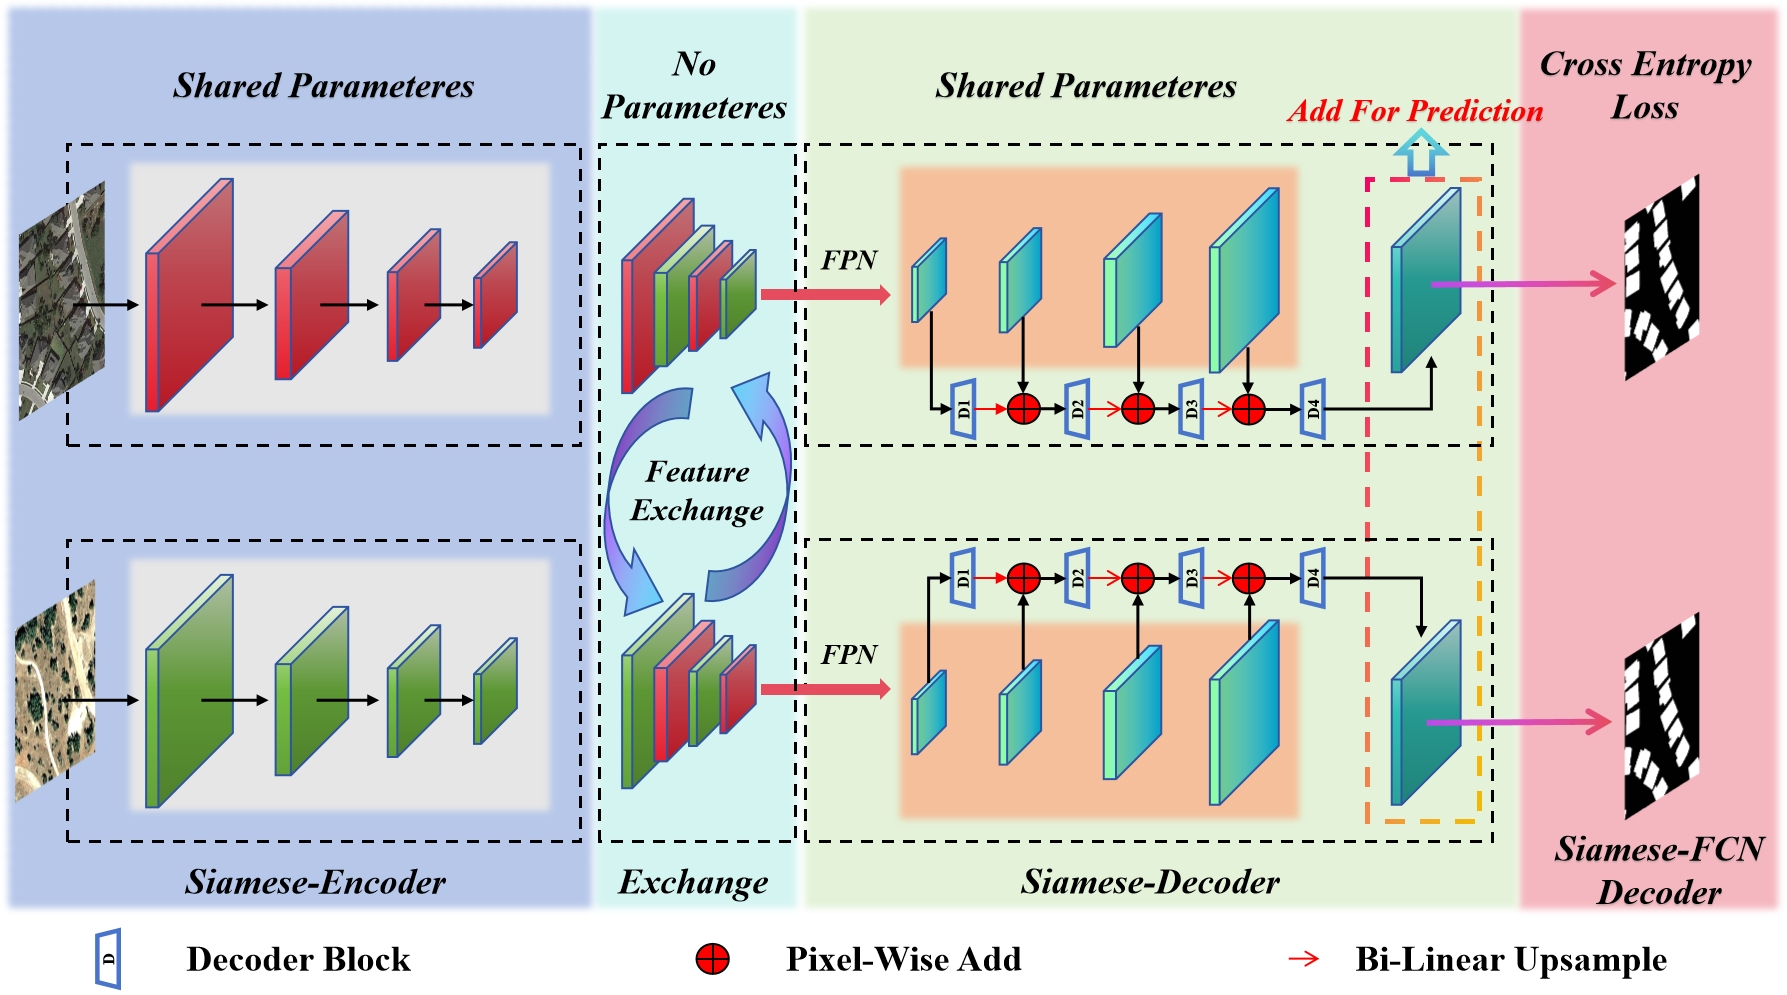
\includegraphics[width=\textwidth]{paper_figures/变化检测任务基础范式设计/SEED_Framework.png}
  \caption{Siamese Encoder-Exchange-Decoder (SEED) 总体架构}
  \label{fig:SEED_Framework}
\end{figure}

\begin{figure}[!htbp]
  \centering
  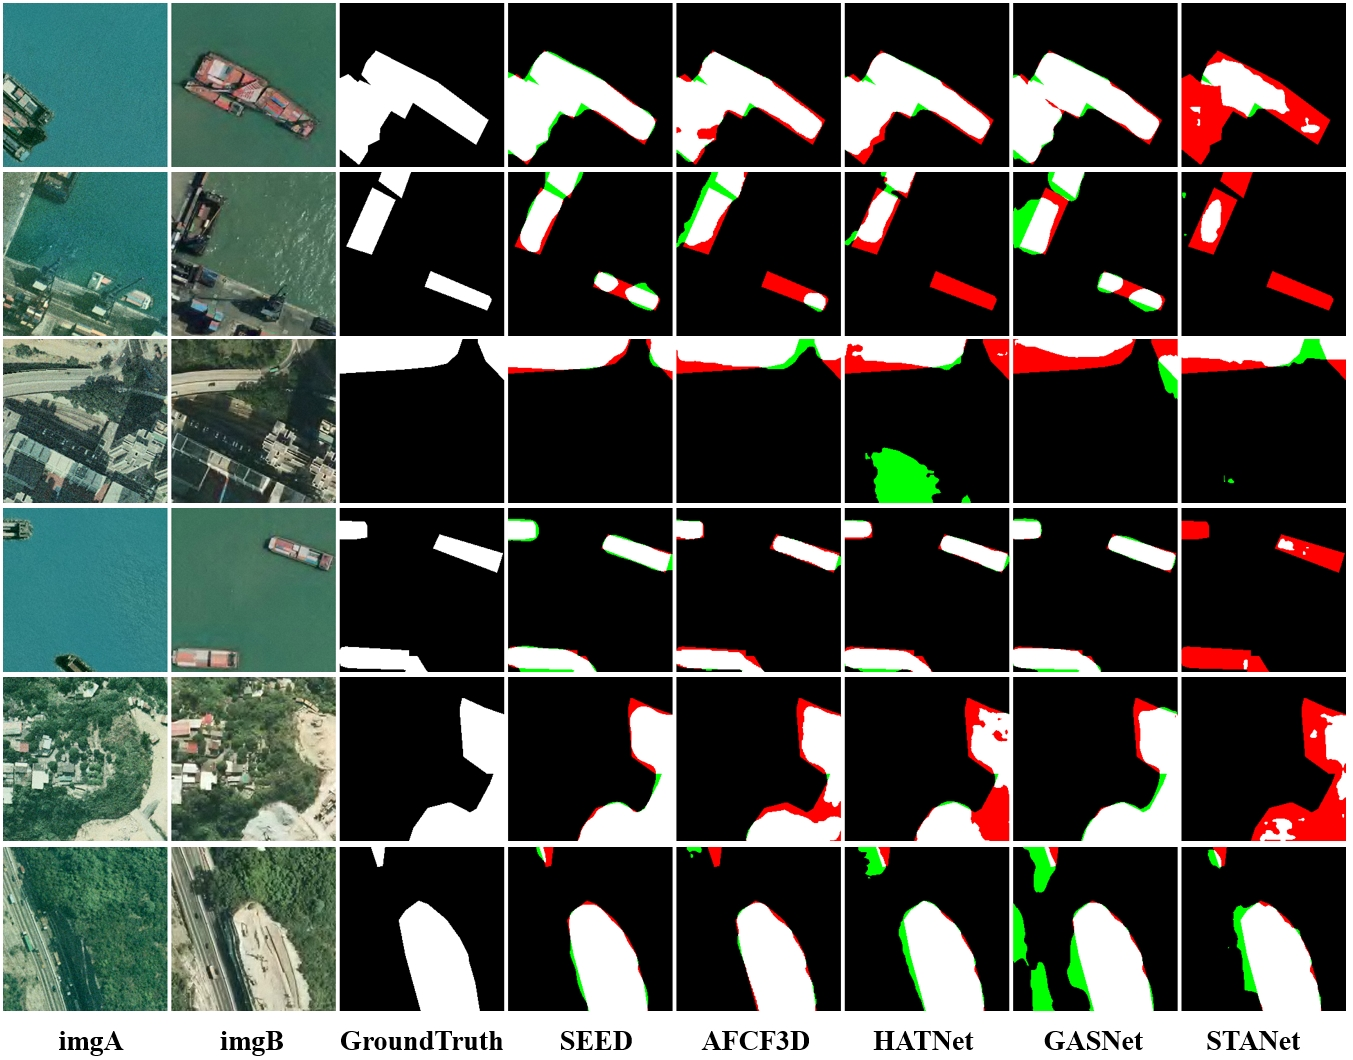
\includegraphics[width=0.8\textwidth]{paper_figures/变化检测任务基础范式设计/seed_sysu.png}
  \caption{ SEED 模型与经典变化检测模型在 SYSU-CD 数据集的可视化对比结果。}
  \label{fig:seed_sysu}
\end{figure}


\begin{table}[!htbp]
\centering
\caption{SEED 模型在 SYSU-CD 数据集上的定量对比结果}
\label{tab:seed_sysu}
\begin{tabular}{lccccc}
\hline
\textbf{Model} & \textbf{OA} & \textbf{IoU} & \textbf{F1} & \textbf{Rec} & \textbf{Prec} \\
\hline
STANet~\cite{chen_spatial-temporal_2020} & 88.24 & 57.22 & 72.79 & 66.71 & 80.08 \\
DSAMNet~\cite{shi_deeply_2022}    & --    & 64.18 & 78.18 & 81.86 & 74.81 \\
P2V~\cite{lin_transition_2023}    & 90.49 & 66.29 & 79.73 & 79.29 & 80.17 \\
RCDT~\cite{lu_cross_2024}         & --    & 67.46 & 80.57 & 86.21 & 75.62 \\
DARNet~\cite{li_densely_2022}     & 91.26 & 68.10 & 81.03 & 79.11 & 83.04 \\
STDF-CD~\cite{y_zhou_stdf_2025}   & 91.42 & 68.83 & 81.53 & 80.35 & 82.76 \\
STFF-GA~\cite{h_wei_spatio-temporal_2024}   & --  & 69.45   & 81.97  & 80.14  & 83.89 \\
SGANet~\cite{j_chen_sganet_2025}  & --    & 69.55 & 82.04 & 76.50 & 88.45 \\
MFCF-Net~\cite{b_huang_remote-sensing_2024}   & 92.05   & 69.79   & 82.21   & 79.37   & 85.25 \\
AMFNet~\cite{zhan_amfnet_2024}     & 92.30  & 69.85 &  82.25 &  82.51 &  88.23 \\
CMCD~\cite{li_cmcd_2025}          & --    & 69.87 & 82.26 & 85.90 & 78.92 \\
MIFNet~\cite{w_xie_mifnet_2025}       & --  & 70.09 & 82.42 & 79.47 & 85.85 \\
\hline
SEED (LE)                             & 92.03 & 70.33 & 82.58 & 80.16 & 85.16 \\
SEED (CE) & 92.16 & 70.91	& 82.98	& 81.01	& 85.05 \\
SEED (SE) & 91.52 & 69.05	& 81.69	& 80.27	& 83.16 \\
\hline
\end{tabular}
\end{table}



\begin{figure}[!htbp]
  \centering
  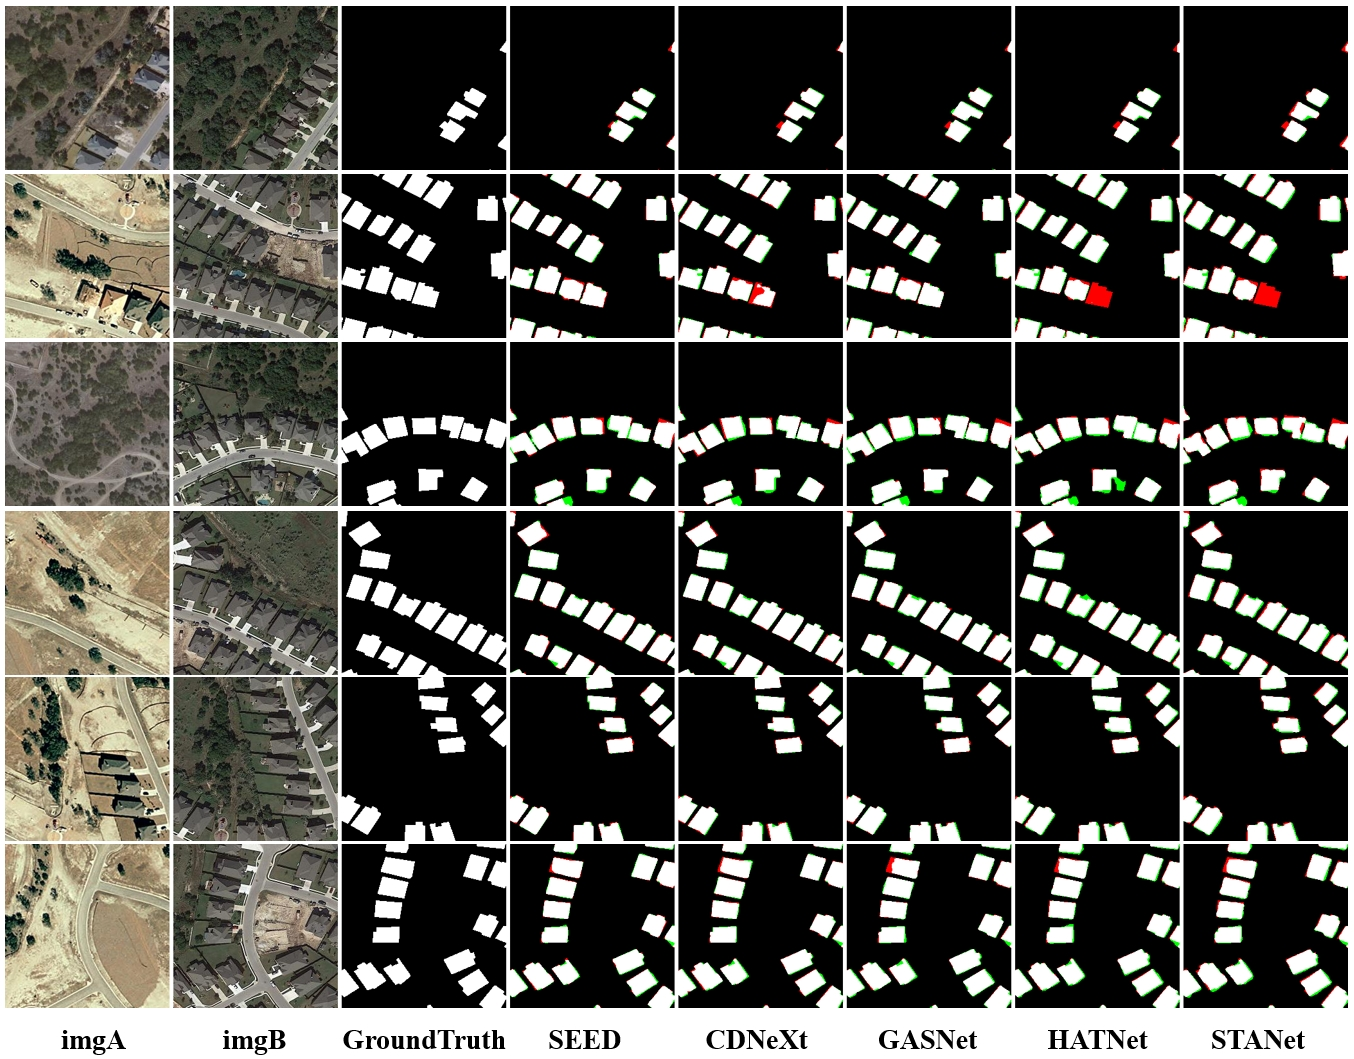
\includegraphics[width=0.8\textwidth]{paper_figures/变化检测任务基础范式设计/seed_levir.png}
  \caption{SEED模型与经典变化检测模型在 LEVIR-CD 数据集的可视化对比结果。}
  \label{fig:seed_levir}
\end{figure}


\begin{table}[!htbp]
\centering
\caption{SEED 模型与经典变化检测模型在 LEVIR-CD 数据集上的定量对比结果}
\label{tab:seed_levir}
\begin{tabular}{lccccc}
\hline
\textbf{Model} & \textbf{OA} & \textbf{IoU} & \textbf{F1} & \textbf{Rec} & \textbf{Prec} \\
\hline
STANet~\cite{chen_spatial-temporal_2020}   & 99.02 & 81.85 & 90.02 & 87.13 & 93.10 \\
CDMamba~\cite{zhang_cdmamba_2025}          & 99.06 & 83.07 & 90.75 & 90.08 & 91.43 \\
AMFNet~\cite{zhan_amfnet_2024}             & 99.07 & 83.13 & 90.79 & 91.15 & 94.77 \\
ISDANet~\cite{h_ren_interactive_2025}      & 99.10 & 83.63 & 91.06 & --    & 92.19 \\
RSM-CD~\cite{zhao_rs-mamba_2024}           & --    & 83.66 & 91.10 & 89.73 & 92.52 \\
DgFA~\cite{f_zhou_dual-granularity_2025}   & 99.11 & 83.93 & 91.26 & 90.84 & 91.69 \\
TRSANet~\cite{j_li_trsanet_2024}           & 99.14 & 84.22 & 91.44 & 89.95 & 92.97 \\
HATNet~\cite{Xu2024HybridAT}             & --    & 84.41 & 91.55 & 90.23 & 92.90 \\
GASNet~\cite{zhang_global-aware_2023}      & 99.11 & --    & 91.21 & 90.62 & 91.82 \\
CMCD~\cite{li_cmcd_2025}                   & --    & 84.50 & 91.60 & 90.48 & 92.74 \\
STFF-GA~\cite{h_wei_spatio-temporal_2024}   & --  & 84.81   & 91.78  & 91.10  & 92.46 \\
MFCF-Net~\cite{b_huang_remote-sensing_2024} & 99.17  & 84.82  & 91.79  & 90.84  & 92.76 \\
STDF-CD~\cite{y_zhou_stdf_2025}            & 99.12 & 85.05 & 91.92 & 91.01 & 92.85 \\
SFFCE-CD~\cite{y_xing_sffce-cd_2025}       & 99.20 & 85.32 & 92.08 & 91.18 & 93.00 \\
MIFNet~\cite{w_xie_mifnet_2025}            & --  & 85.35 & 92.10 & 90.87 & 93.37 \\
SGANet~\cite{j_chen_sganet_2025}           & --    & 85.45 & 92.14 & 91.03 & 93.30 \\
RCDT~\cite{lu_cross_2024}                  & --    & 85.50 & 92.18 & 93.27 & 91.12 \\
FTA-Net~\cite{t_zhu_fta-net_2025}          & --    & 85.58 & 92.23 & 92.68 & 91.79 \\
CDNeXt~\cite{wei_robust_2024}              & 99.24 & 85.86 & 92.39 & 90.92 & 93.91 \\
HASNet~\cite{c_tao_hasnet_2025}            & 99.53 & 85.90 & 92.42 & 92.04 & 92.80 \\
UA-BCD~\cite{li_overcoming_2025}           & --    & 85.99 & 92.47 & 91.57 & 93.38 \\
FTransDF-Net~\cite{li_dual_2025}           & --    & 86.04 & 92.50 & 91.40 & 93.62 \\
RSBuilding~\cite{wang_rsbuilding_2024}     & --    & 86.19 & 92.59 & 91.80 & 93.39 \\
\hline
SEED (LE)                                      & 99.26 & 86.25 & 92.62 & 90.97 & 94.32 \\
SEED (CE) & 99.25	& 86.03	& 92.49	& 91.08	& 93.94 \\
SEED (SE) & 99.26	& 86.24	& 92.61	& 91.42	& 93.83 \\
\hline
\end{tabular}
\end{table}

\section{SEED架构设计方法}
\subsection{整体架构}  
本工作主要探讨变化检测任务的框架设计~\cite{dong_efficientcd_2024, Fang2022ChangerFI, zhao_exchanging_2023},提出了 Siamese Encoder-Exchange-Decoder(SEED)框架,如图~\ref{fig:SEED_Framework} 所示。在 SEED 框架的编码阶段,基于 SwinTv2-Base~\cite{liu_swin_2021-5}、EfficientNet-B4~\cite{tan_efficientnet_2019} 和 ResNet50~\cite{He2015DeepRL} 构建了权重共享的 Siamese 编码器。在特征交换阶段,采用了三种不同的交换方式:特征图层交换、特征图通道交换和特征图空间交换。在颈部阶段,使用参数共享的特征金字塔网络(FPN)~\cite{lin_feature_2017} 对交换后的双时相特征金字塔进行处理。在解码阶段,为了充分验证 SEED 框架的潜力,构建了一个极其简洁的逐层解码结构,并共享解码器参数。此外,对于 SwinTv2 主干网络,在解码器中集成了简单的 Swin Transformer V2 模块以优化特征;而对于 EfficientNet 和 ResNet,则采用 ResNet 的 BottleNeck 模块进行特征优化。在训练阶段,解码器的两个分支分别计算损失;在推理阶段,将两个分支的预测结果相加并取平均,作为变化检测模型的最终输出。

\subsection{特征交换方法}  
在前人工作~\cite{dong_efficientcd_2024, Fang2022ChangerFI, zhao_exchanging_2023}的基础上,本章深入研究了三种特征交换方案,并通过实验结果验证了变化检测任务中的像素一致性定理。首先,这些方案在不引入任何额外可学习参数的条件下,即可促进双时相影像间的特征信息交互,增强模型对双时相数据的理解;其次,基于这些特征交互的框架摒弃了复杂的差异特征计算,使模型在保留原始特征完整性的同时,学习到有效的变化特征。以下分别介绍这三种方案。

\subsubsection{特征图层交换(Layer-Exchange, LE)}
特征图层交换在层级维度上进行特征交换,如图~\ref{fig:seed_exchange}(a) 所示。给定来自双时相影像的两组特征列表 \(\{x_i\}\) 和 \(\{y_i\}\),按照预设步长(例如每隔一层)交换对应层的特征。具体而言,假设特征列表为 \(\{x_0, x_1, x_2, x_3\}\) 与 \(\{y_0, y_1, y_2, y_3\}\),则以步长 \(2\) 交换 \(x_0 \leftrightarrow y_0\)、\(x_2 \leftrightarrow y_2\),其余层保持不变。

\subsubsection{特征图通道交换(Channel-Exchange, CE)} 
特征图通道交换按固定规则交换通道,如图~\ref{fig:seed_exchange}(b) 所示。例如,在通道交换中,依据预设步长(如 $2$)选择部分通道进行交换。假设共有 $C$ 个通道,则依次交换通道索引为 $0,2,4,\ldots$ 的通道与另一路分支的对应通道,其余通道保持不变。


\begin{figure}[!htbp]
  \centering
  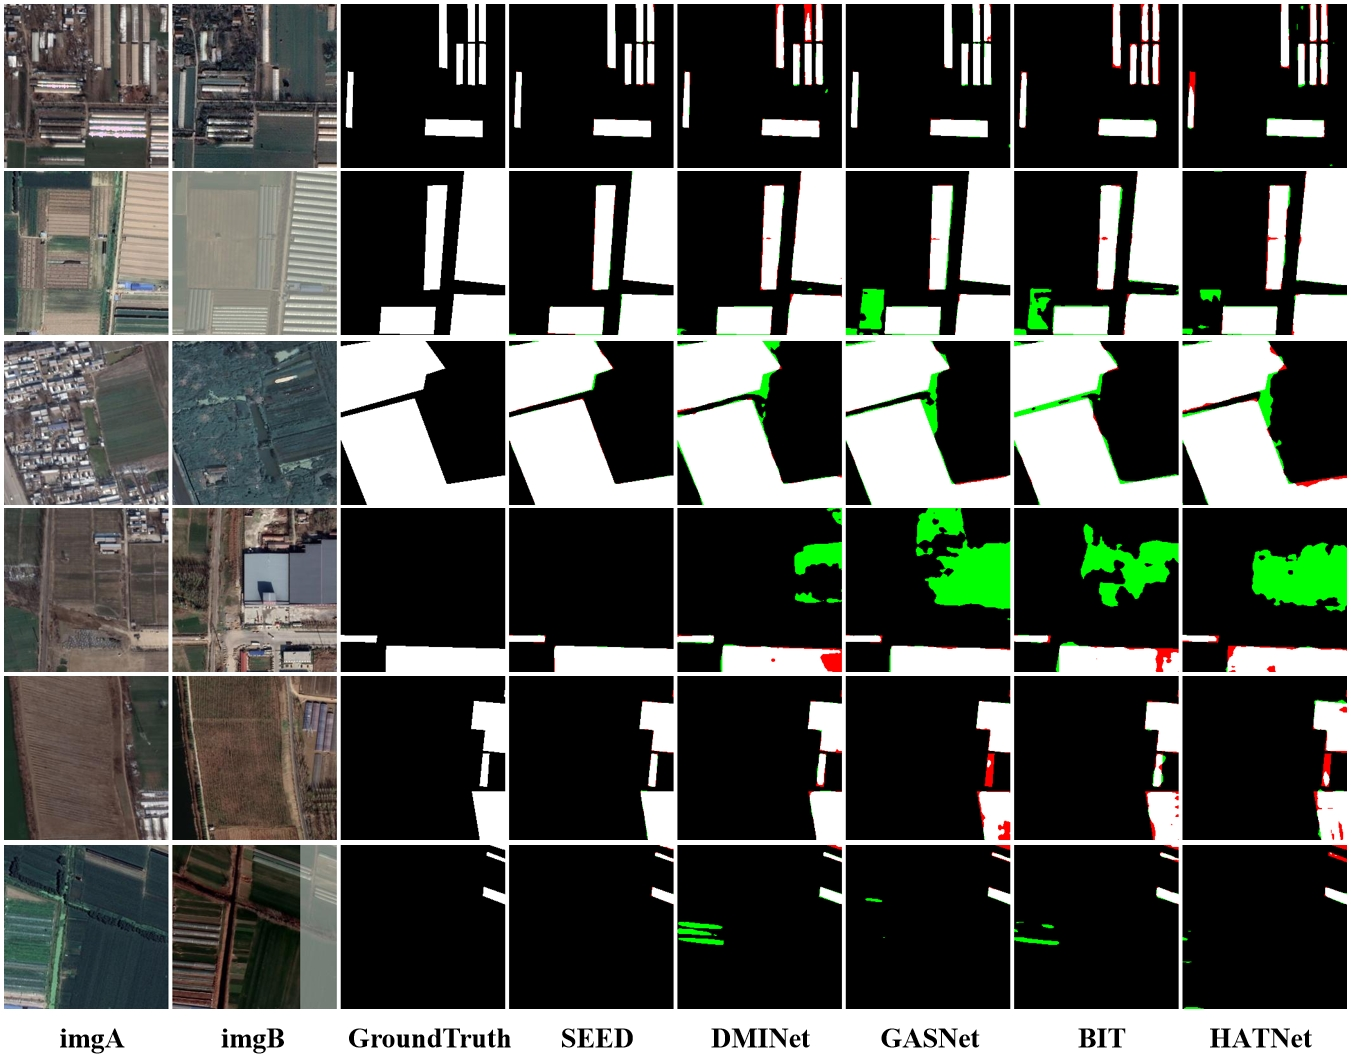
\includegraphics[width=0.8\textwidth]{paper_figures/变化检测任务基础范式设计/seed_pxclcd.png}
  \caption{SEED 模型与经典变化检测模型在 PX-CLCD 数据集的可视化对比结果。}
  \label{fig:seed_pxclcd}
\end{figure}

\subsubsection{特征图空间交换(Spatial-Exchange, SE)}
特征图空间交换在空间维度上进行特征交换,如图~\ref{fig:seed_exchange}(c) 所示。具体而言,给定双时相影像的两幅特征图,按照预设步长(例如 $2$)在宽度(或高度)方向上按指定间隔将特征图划分为若干列(或行),并交换两幅特征图中对应的列(或行)。


\begin{table}[!htbp]
\centering
\caption{SEED 模型与经典变化检测模型在 PX-CLCD 数据集上的定量对比结果}
\label{tab:seed_pxclcd}
\begin{tabular}{lccccc}
\hline
\textbf{Model} & \textbf{OA} & \textbf{IoU} & \textbf{F1} & \textbf{Rec} & \textbf{Prec} \\
\hline
HANet~\cite{Han2024HANetAH}         & 98.50 & 88.99 & 94.18 & 93.83 & 94.53 \\
MSCANet~\cite{m_liu_cnn-transformer_2022}       & 98.50 & 89.00 & 94.18 & 93.95 & 94.41 \\
DDAM-Net~\cite{feng_ddam-net_2024} & -- & 90.70 & 95.12 & 94.78 & 95.47 \\
BIT~\cite{chen_remote_2022}           & 98.76 & 90.78 & 95.17 & 94.80 & 95.54 \\
GASNet~\cite{zhang_global-aware_2023}    & 98.99 & 92.51 & 96.11 & 96.42 & 95.80 \\
DMINet~\cite{feng_change_2023}         & 99.04 & 92.83 & 96.28 & 96.31 & 96.25 \\
SNUNet3+~\cite{miao_snunet3_2024}     & 99.19 & 93.61 & 96.64 & 96.79 & 96.60 \\
CGNet~\cite{han_change_2023}         & 99.17 & 93.82 & 96.81 & 97.33 & 96.30 \\
\hline
SEED (LE)          & 99.38 & 95.34 & 97.61 & 97.46 & 97.76 \\
SEED (CE)          & 99.40	& 95.50	& 97.70	& 98.07	& 97.33 \\
SEED (SE)          & 99.32 & 94.86 & 97.36 & 96.89 & 97.84 \\
\hline
\end{tabular}
\end{table}

\subsubsection{随机交换(Random Exchange)}
为了进一步验证特征交换方法的有效性及像素一致性原则在变化检测任务中的正确性,在上述三种特征交换方法的基础上引入随机性,提出了一种随机交换策略,以在训练过程中实现更丰富的特征混合。具体而言,随机交换不再按照固定规则(如固定步长或索引)进行特征交换,而是基于一定的概率或随机选择策略,在不同层级、通道或空间位置有选择地交换特征,具体如下:

\textbf{随机层交换(Random Layer Exchange, RLE)}: 对每一层生成一个随机数;若该随机数小于给定阈值(例如 0.5),则交换对应层的特征,否则保持不变。

\textbf{随机通道交换(Random Channel Exchange, RCE)}: 首先随机打乱通道索引,然后按一定比例(例如 0.5)选择部分通道进行交换,其余通道保持不变。

\textbf{随机空间交换(Random Spatial Exchange, RSE)}: 在空间维度上,对每个位置(如列或行)生成一个随机数,并以一定概率(例如 0.5)决定是否交换该位置的特征。  



\begin{figure}[!htbp]
  \centering
  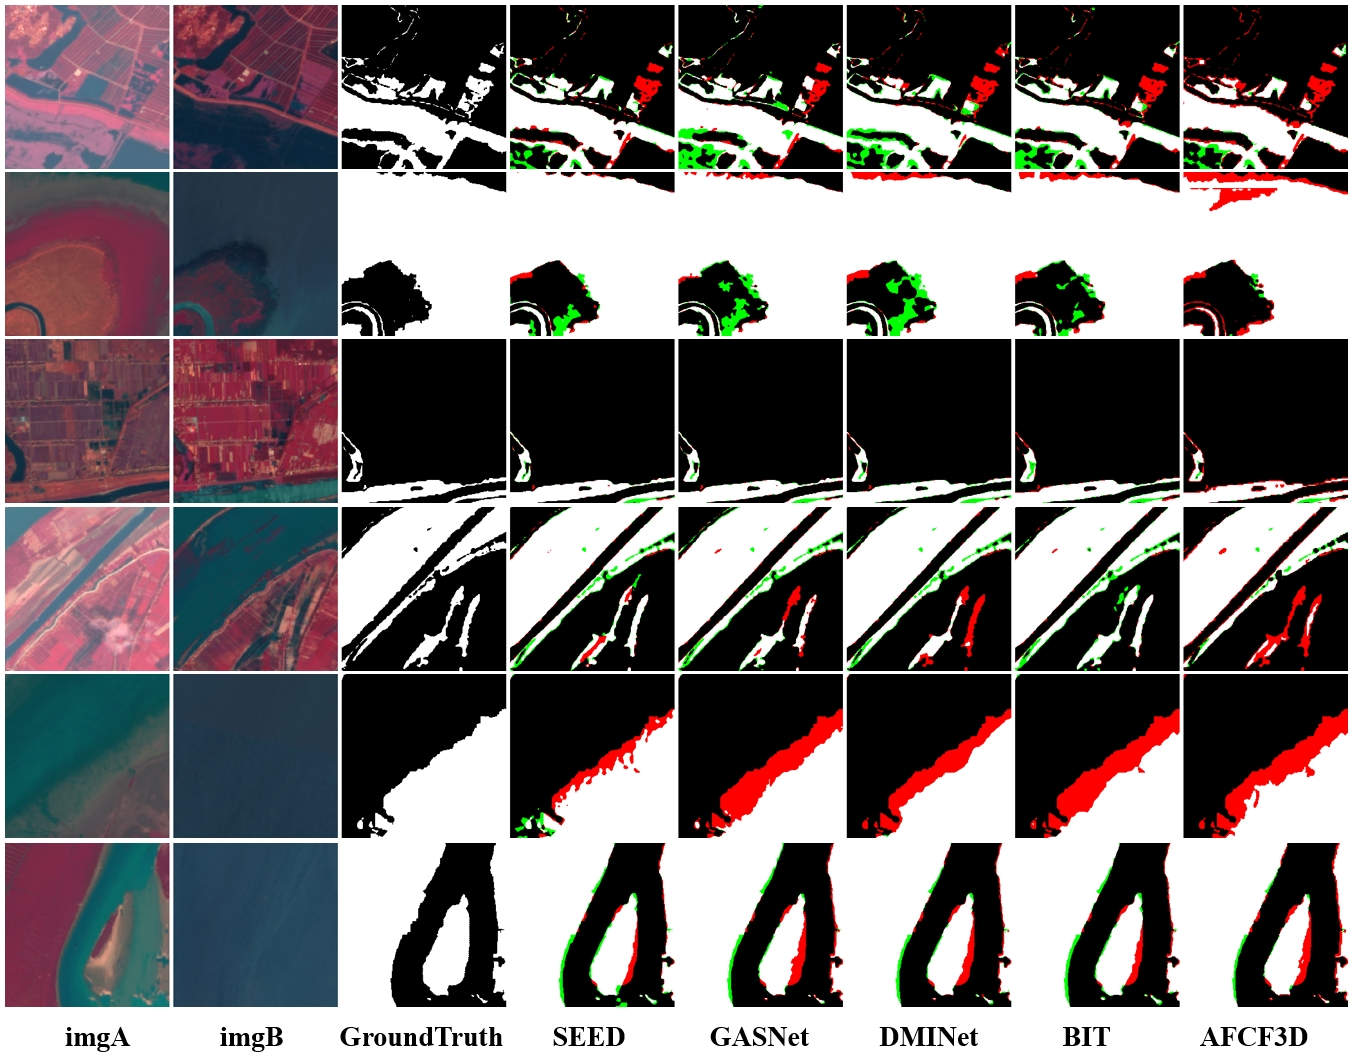
\includegraphics[width=0.8\textwidth]{paper_figures/变化检测任务基础范式设计/seed_watercd.png}
  \caption{SEED 模型与经典变化检测模型在 Water-CD 数据集的可视化对比结果}
  \label{fig:seed_watercd}
\end{figure}

使用上述特征交换方案进行了大量实验。结果表明,这些方案均未对变化检测模型的性能产生负面影响。在随机交换实验中,传统计算机视觉通常将通道信息与语义内容关联、将空间信息与纹理关联,因此对其进行更改时往往需要谨慎。然而在变化检测任务中,可以按照特定规则交换特征图,甚至采用随机交换策略。这一现象验证了变化检测任务中的像素一致性原则。实验结果表明,基于深度学习的变化检测模型并不依赖于构建差异特征,而是通过特征交换直接从双时相特征中学习变化区域的特征。


\begin{table}[!htbp]
\centering
\caption{SEED 模型与经典变化检测模型在 Water-CD 数据集上的定量对比结果}
\label{tab:seed_watercd}
\begin{tabular}{lccccc}
\hline
\textbf{Model} & \textbf{OA} & \textbf{IoU} & \textbf{F1} & \textbf{Rec} & \textbf{Prec} \\
\hline
AFCF3DNet~\cite{ye_adjacent-level_2023} & 95.63 & 77.06 & 87.04 & 80.17 & 95.20 \\
HANet~\cite{Han2024HANetAH}    & 95.94 & 79.94 & 88.85 & 88.34 & 89.37 \\
ELGCNet~\cite{m_noman_elgc-net_2024}   & 96.14 & 80.79 & 89.37 & 88.60 & 90.16 \\
BIT~\cite{chen_remote_2022}           & 96.52 & 82.52 & 90.42 & 89.55 & 91.31 \\
DMINet~\cite{feng_change_2023}         & 96.55 & 82.67 & 90.51 & 89.87 & 91.17 \\
GASNet~\cite{zhang_global-aware_2023}    & 96.72 & 83.48 & 91.00 & 90.41 & 91.59 \\
CDNeXt~\cite{wei_robust_2024}        & 96.88 & 84.21 & 91.43 & 90.71 & 92.15 \\
TRSANet~\cite{j_li_trsanet_2024}     & 97.01 & 84.69 & 91.71 & 90.22 & 93.25 \\
\hline
SEED (LE)          & 96.98 & 84.64 & 91.68 & 90.69 & 92.69 \\
SEED (CE) & 96.94	& 84.43	& 91.56	& 90.64	& 92.50 \\
SEED (SE) & 96.86	& 84.06	& 91.34	& 90.42	& 92.27 \\
\hline
\end{tabular}
\end{table}


\subsection{孪生-编码-交换-解码(SEED)框架设计原理}
尽管在语义分割任务中,特征交换方案可能会破坏图像特征,但在变化检测任务中,只要双时相影像中成对像素的空间对应关系得以保持,无论如何交换特征,模型的学习目标均保持不变。本章将双时相影像中对应像素对的空间关系保持称为“像素一致性原则”。换言之,只要遵循像素一致性原则,任何形式的特征交换都不会影响变化检测模型的基本性能。因此,在保持像素一致性的前提下,可基于多种特征交换规则设计灵活的变化检测模型。  


\begin{figure}[!htbp]
  \centering
  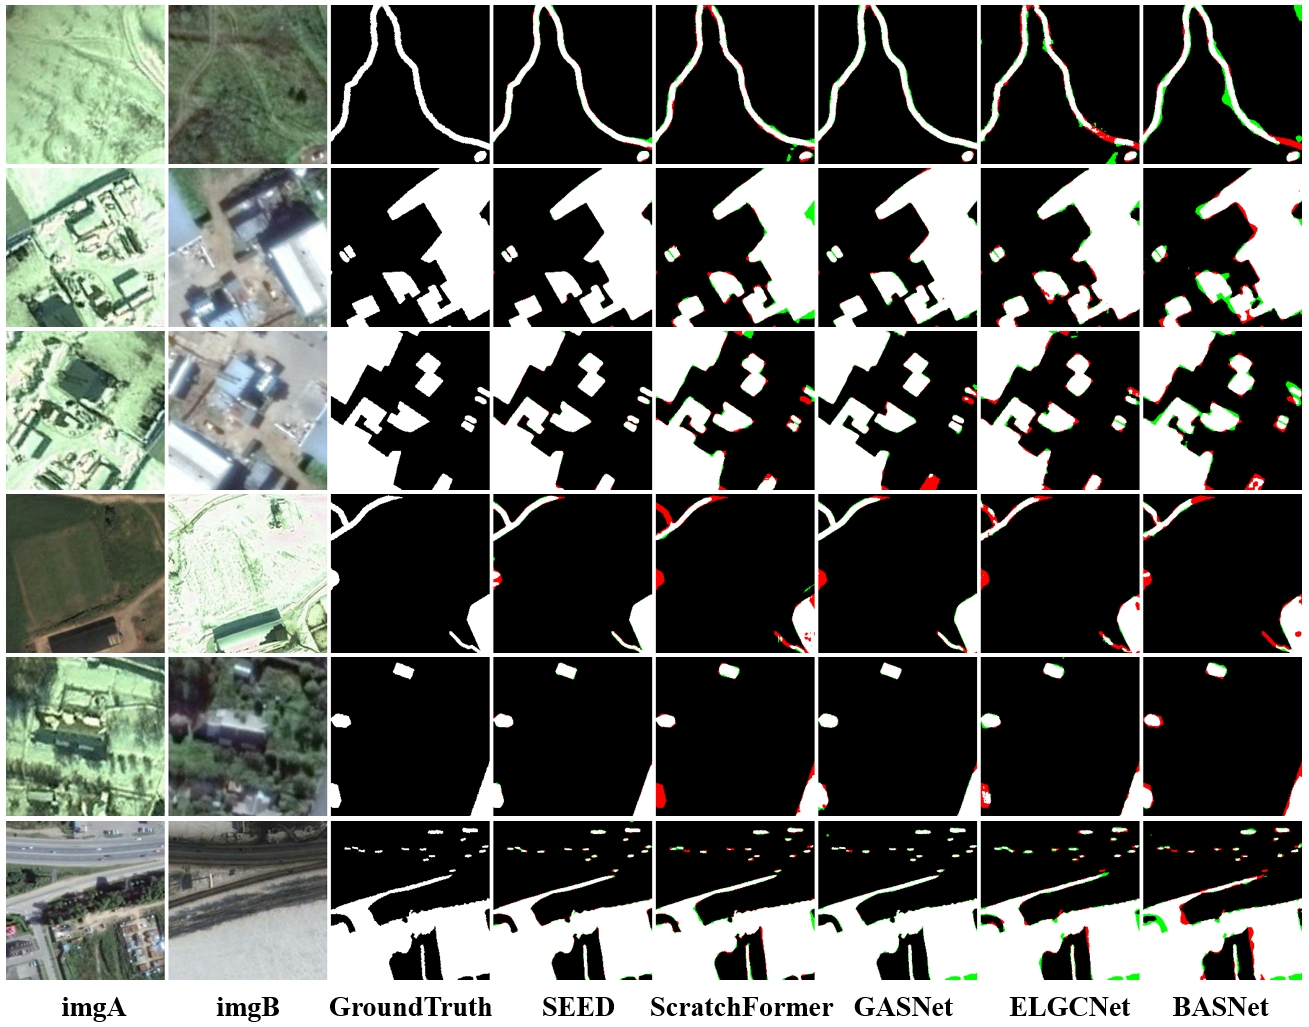
\includegraphics[width=0.8\textwidth]{paper_figures/变化检测任务基础范式设计/seed_cdd.png}
  \caption{SEED 模型与经典变化检测模型在 CDD 数据集的可视化对比结果}
  \label{fig:seed_cdd}
\end{figure}

基于上述特征,设计了如图~\ref{fig:SEED_Framework} 所示的方案。采用常见的主干网络作为编码器进行特征提取,并实现了权重共享的双分支结构。特征提取完成后,加入特征交换阶段,并分别对前文讨论的三种特征交换方案进行实验验证。随后,将经过特征交换的双时相特征金字塔输入参数共享的特征金字塔网络(FPN)进行进一步处理。FPN 模块通过融合与信息交换,实现了双分支特征金字塔的全面融合,等效地将两条分支转换为两组等价的特征金字塔序列。最后,基于这两组特征金字塔,设计了一个基于逐层上采样的简单特征融合解码器作为基础解码方案。此外,由于经过特征交换后 FPN 处理的双时相特征金字塔在本质上是等价的,因此在解码阶段同样采用了参数共享的解码器。基于上述 SEED 框架的构建,仅使用一套编码器—解码器参数,即可构建出高性能的变化检测模型。  


\begin{table}[!htbp]
\centering
\caption{SEED 模型与经典变化检测模型在 CDD 数据集上的定量对比结果}
\label{tab:seed_cdd}
\begin{tabular}{lccccc}
\hline
\textbf{Model} & \textbf{OA} & \textbf{IoU} & \textbf{F1} & \textbf{Rec} & \textbf{Prec} \\
\hline
BASNet~\cite{z_wang_bitemporal_2024} & 99.18 & 93.29 & 96.53 & 96.30 & 96.76 \\  
UA-BCD~\cite{li_overcoming_2025}     & --    & 93.49 & 96.64 & 96.90 & 96.38 \\
RCDT~\cite{lu_cross_2024}                  & --    & 93.79 & 96.80 & 96.97 & 96.63 \\
CDMamba~\cite{zhang_cdmamba_2025}    & 99.26 & 93.93 & 96.87 & 96.84 & 96.90 \\
SFFCE-CD~\cite{y_xing_sffce-cd_2025}   & 99.29 & 94.42 & 97.13 & 96.94 &  97.32 \\
ELGCNet~\cite{m_noman_elgc-net_2024}   & 99.33  &  94.50   & 91.17  & --   & -- \\   
DgFA~\cite{f_zhou_dual-granularity_2025} & 99.41 & 95.12 & 97.50 & 97.60 & 97.40 \\
GASNet~\cite{zhang_global-aware_2023}  & 99.41  & 95.34  & 97.61  & 98.06  & 97.17 \\
MLDFNet~\cite{d_sidekejiang_mldfnet_2025}  & -- & 95.78 & 97.84 & 97.97 & 97.72 \\
ScratchFormer~\cite{Noman2023RemoteSC}   & 99.50 & 95.85  & 97.88 & -- & -- \\ 
FTransDF-Net~\cite{li_dual_2025}   & -- & 95.85 &  97.88 & 97.63 & 98.13 \\
DSFI-CD~\cite{x_li_dsfi-cd_2025}  & 99.52 & 96.10 &  98.01 & 98.34 & 97.68 \\
HASNet~\cite{c_tao_hasnet_2025}        & 99.56 & 96.49 & 98.21 & 98.12 & 98.32 \\
\hline
SEED (LE)                               & 99.64	& 97.11	& 98.53	& 98.44	& 98.63 \\
SEED (CE) & 99.59	& 96.75	& 98.35	& 98.36	& 98.34 \\
SEED (SE) & 99.55	& 96.40	& 98.17	& 98.02	& 98.32 \\
\hline
\end{tabular}
\end{table}


\section{实验结果与分析}

\subsection{实验结果量化指标与可视化分析}
在本章中,对 SEED 架构与最先进的变化检测算法进行了详细的对比实验。表中所有 SEED 的结果均基于 Swin Transformer V2 主干网络。正如表~\ref{tab:seed_sysu}、表~\ref{tab:seed_levir}、表~\ref{tab:seed_pxclcd}、表~\ref{tab:seed_watercd}和表~\ref{tab:seed_cdd} 所示,SEED 框架在SYSU-CD、LEVIR-CD、PX-CLCD、Water-CD 以及 CDD数据集上均表现优异,充分展示了其有效性和鲁棒性。此外,无论是层交换(LE)、通道交换(CE)还是空间交换(SE),SEED 架构的各项准确率指标均十分出色,进一步验证了特征交换方法的合理性。


\begin{figure}[!htbp]
    \centering
    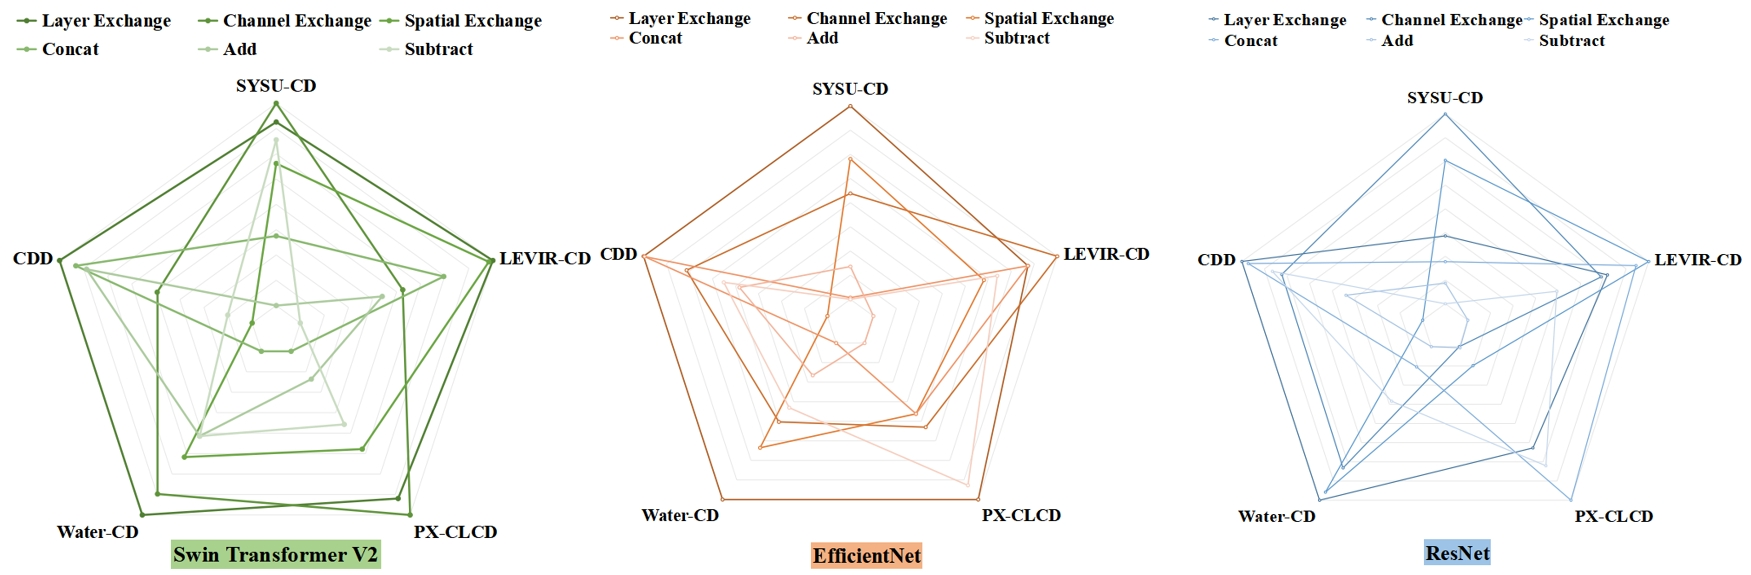
\includegraphics[width=\textwidth]{paper_figures/变化检测任务基础范式设计/seed_rader_image.png} % 
    \caption{基于IoU指标的SEED 架构配合不同特征交换方法在变化检测数据集上的对比结果}
    \label{fig:seed_rader_image}
\end{figure}

首先,在 SYSU‐CD 数据集上,SEED 模型实现了 92.16\% 的整体准确率(OA)和 70.91\% 的 IoU,F1 分数为 82.98\%。这不仅显著超过了 DSAMNet、P2V、DARNet 和 STDF‐CD 等模型,而且在 Recall 与 Precision 上表现均衡,表明 SEED 即使在复杂场景中也能有效捕捉双时相影像中的细微变化。

其次,在以建筑变化检测为主的 LEVIR‐CD 数据集上,大多数模型已取得较高分数,但 SEED 仍以 99.26\% 的 OA 和 86.25\% 的 IoU 排名第一。与在更大建筑数据集上训练的 RSBuilding 模型相比,SEED 在 F1 与 Precision 上虽优势有限却稳定,展现了其在建筑变化检测任务中准确识别变化区域的卓越能力。

在以耕地变化检测为主且需要提取细节的 PX‐CLCD 数据集上,SEED 模型取得了 99.40\% 的 OA、95.50\% 的 IoU 以及 97.70\% 的 F1 分数,远超 SNUNet3+、CGNet 等其他模型。该结果证明 SEED 框架具备更强的细节提取与区分能力,更加适用于复杂耕地变化检测场景。  


\begin{figure}[!htbp]
    \centering
    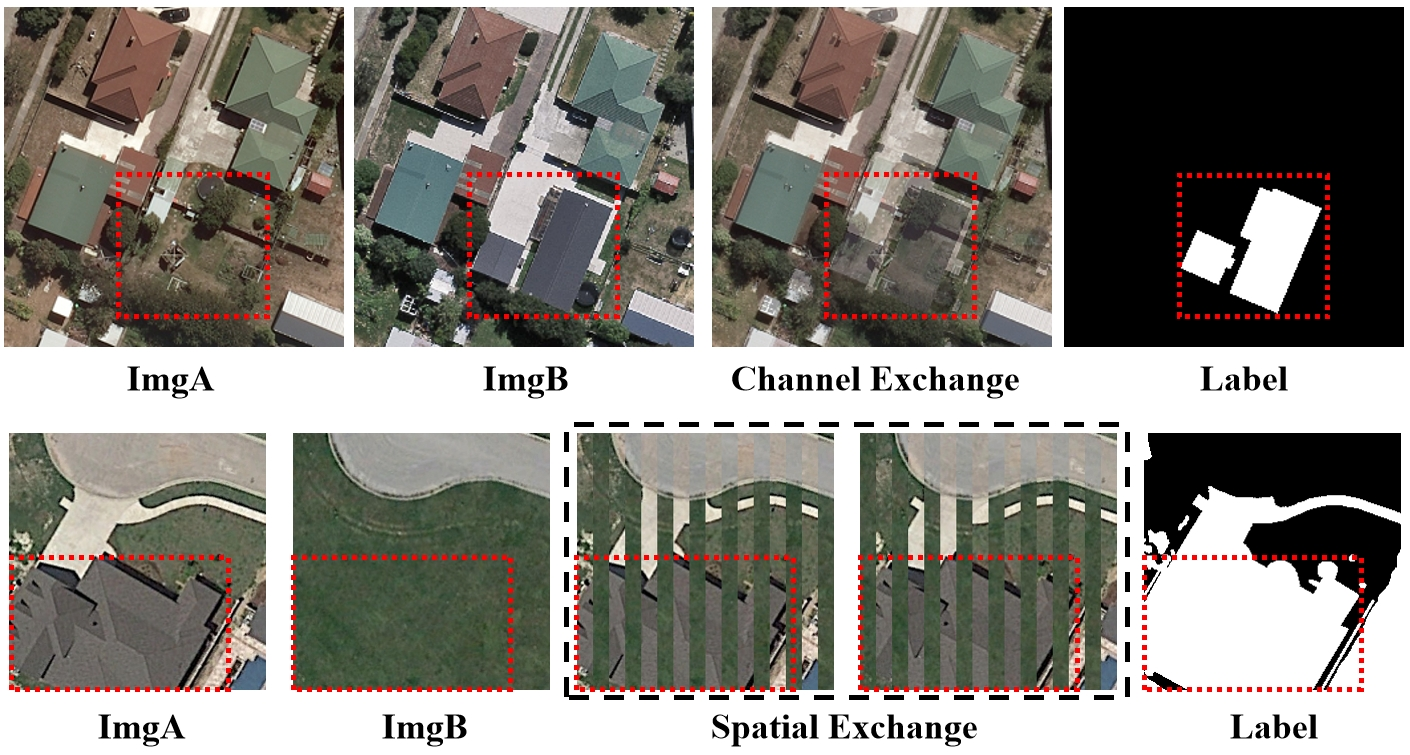
\includegraphics[width=\textwidth]{paper_figures/变化检测任务基础范式设计/seed_exchange_vis.png} % 
    \caption{针对于原始图像的特征交换的可视化结果,突出显示了变化区域。}
    \label{fig:seed_exchange_vis}
\end{figure}

\begin{figure}[!htbp]
  \centering
    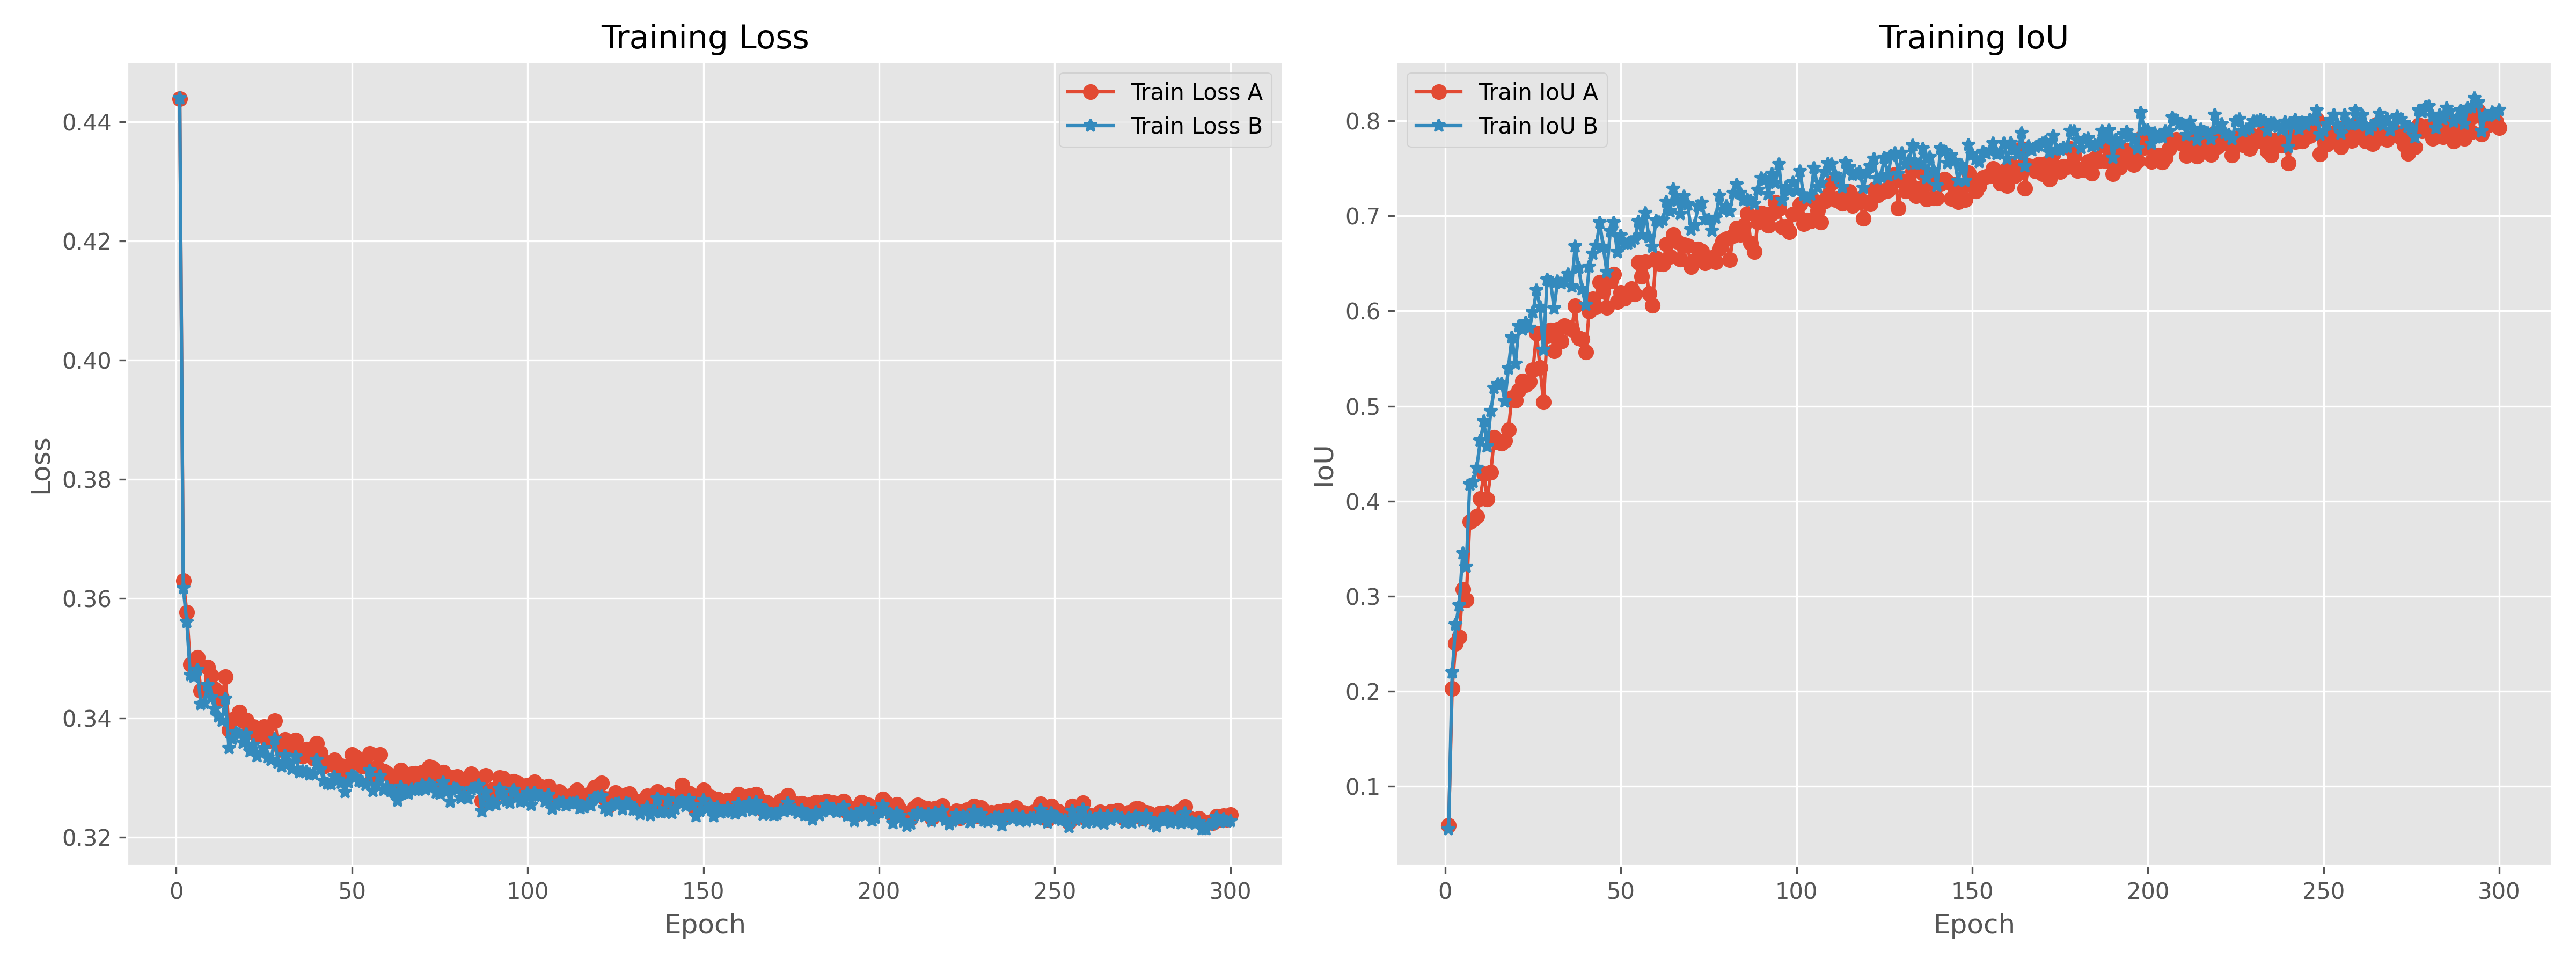
\includegraphics[width=0.8\textwidth]{paper_figures/变化检测任务基础范式设计/chanel_training_log.png} % 
    \caption{基于通道交换的训练日志}
    \label{fig:chanel_training}
\end{figure}
  
\begin{figure}[!htbp]
    \centering
    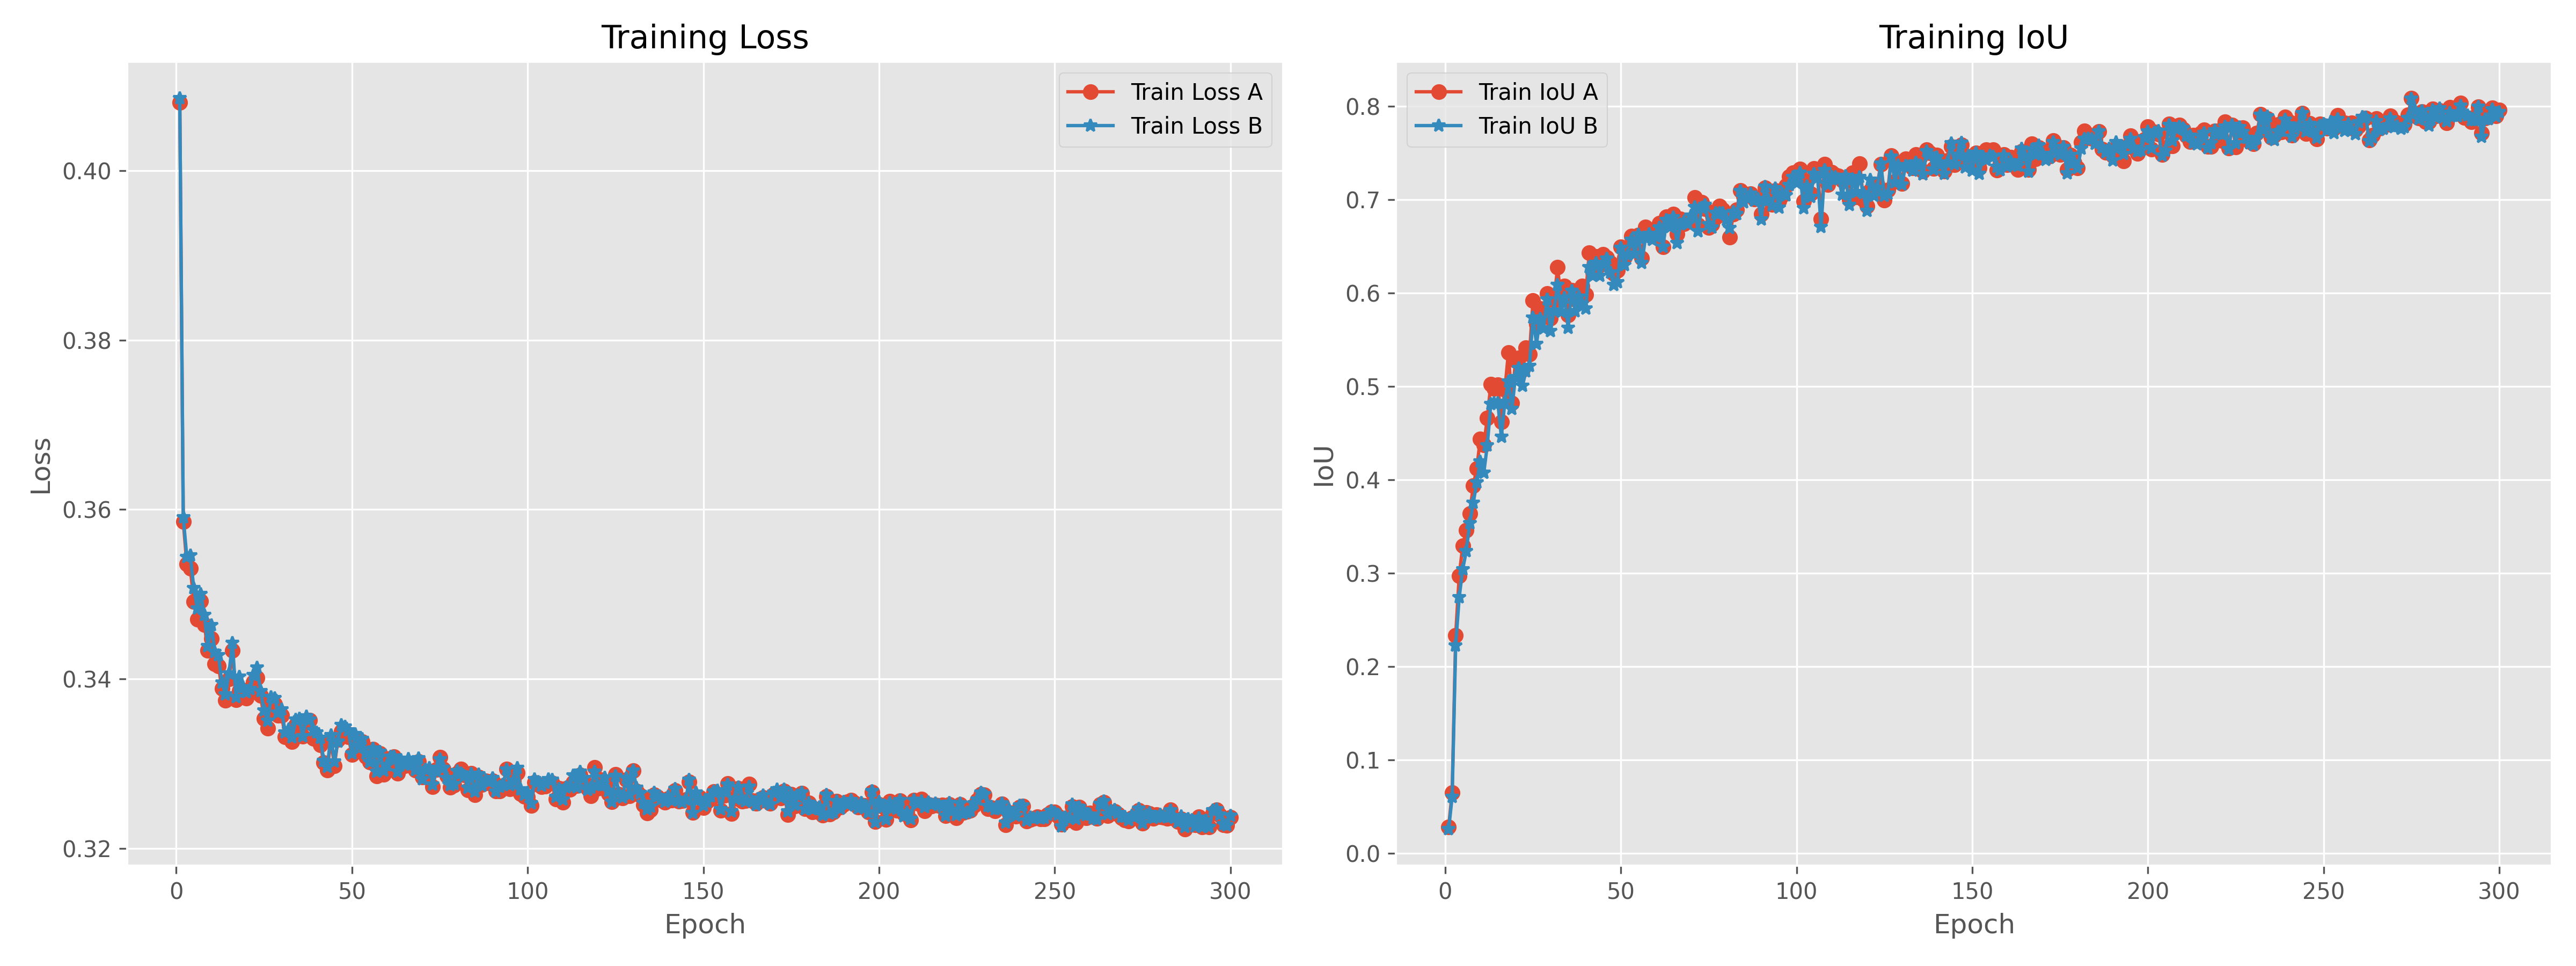
\includegraphics[width=0.8\textwidth]{paper_figures/变化检测任务基础范式设计/spatial_training_log.png} % 
    \caption{基于空间交换的训练日志}
    \label{fig:spatial_training}
\end{figure}

首先,在 Water-CD 数据集上,SEED 模型仍取得了 96.98\% 的整体准确率(OA)和 84.64\% 的 IoU,F1 分数为 91.68\%,在所有指标上均超越了 AFCF3DNet、HANet 和 ELGCNet 等方法。这表明 SEED 框架能够有效处理水资源变化检测中固有的复杂特征,具有很高的实用价值。

最后,在面向季节变化且需要高精度捕捉细微连续变化的 CDD 数据集上,SEED 模型表现卓越,以 99.64\% 的 OA、97.11\% 的 IoU 和 98.53\% 的 F1 分数领先所有对比模型,展现了极高的检测准确性和稳定性。

总体而言,SEED 框架通过摒弃传统的差异特征计算方法,而将特征交换与简洁的编码器–解码器结构相结合,不仅在各类场景和数据集上取得了优异性能,还在建筑变化、耕地变化、水资源变化和季节变化等应用中展现了强大的适应性和鲁棒性。这些实验结果充分验证了特征交换策略在变化检测任务中的有效性。

此外,图~\ref{fig:seed_sysu}、图~\ref{fig:seed_levir}、图~\ref{fig:seed_pxclcd}、图~\ref{fig:seed_watercd}和图~\ref{fig:cdd} 展示了 SEED 模型在 SYSU-CD、LEVIR-CD、PX-CLCD、Water-CD 和 CDD 等五个数据集上的测试结果可视化。这些数据集代表了多种变化检测场景:SYSU-CD 涵盖多目标变化,LEVIR-CD 主要关注建筑物变化,PX-CLCD 强调耕地变化,Water-CD 聚焦水体变化,而 CDD 则反映季节性变化特征。在这些可视化图像中,真阳性(TP)以白色像素表示,真阴性(TN)以黑色像素表示,假阳性(FP)以绿色像素表示,假阴性(FN)以红色像素表示。直观的可视化结果表明,SEED 模型能够在多种场景中准确捕捉变化区域,其检测结果与真实标注高度一致,不仅具有极高的检测精度,还展现了出色的鲁棒性和稳定性。这些丰富的可视化进一步验证了 SEED 框架在处理各类变化类型和复杂环境中的卓越性能。

\subsection{消融研究}
在本章中,提出了一种新颖的变化检测框架——SEED 架构。该框架完全摒弃了变化检测任务中常用的差异特征计算模块,而仅在双时相特征金字塔上应用特征交换。如表~\ref{tab:seed_sysu_backbone} 至表~\ref{tab:seed_cdd_backbone} 所示,在 SYSU-CD、LEVIR-CD、PX-CLCD、Water-CD 和 CDD 数据集上进行了实验。特征提取阶段,分别采用 Swin Transformer V2、EfficientNet-B4 和 ResNet50 作为主干网络;特征交换阶段,依次应用了层交换、通道交换和空间交换三种方法;解码设计中,对于基于 Swin Transformer V2 的主干,使用 Swin Transformer Block 构建解码器;对于 EfficientNet-B4 与 ResNet50 主干,采用 ResNet 的 BottleNeck 模块进行特征优化。为与传统差异特征构建方法比较,还选取了拼接、相加和相减三种方法作为基线。实验结果表明,在大多数条件下,结合特征交换的 SEED 框架性能均优于基于传统差异特征构建方法的变化检测框架。图~\ref{fig:seed_rader_image} 展示了基于 IoU 指标绘制的多个实验结果雷达图:深色指标代表采用特征交换的实验,浅色指标代表依赖传统差异学习的实验。可以看到,深色结果始终更靠近图的外圈,表明基于特征交换的变化检测架构较传统差异特征学习架构具有更优的性能。

此外,计算了层交换、通道交换、空间交换、拼接、相加和相减六种方法的参数量。如表~\ref{tab:seed_params_gflops} 所示,特征交换方法所需参数量与相加和相减方法一致,且略低于拼接方法。这进一步证实,SEED 框架在参数配置上与传统差异特征构建方法保持一致,并且由于其简洁的架构,能够在变化检测任务中取得卓越的性能。


\begin{table}[!htbp]
\centering
\caption{基于 SEED 架构结合不同主干网络以及多种特征交换机制在 SYSU-CD 数据集上的测试结果}
\label{tab:seed_sysu_backbone}
\begin{tabular}{l l c c c c c}
\hline
\textbf{Backbone} & \textbf{Exchange Method} & \textbf{OA} & \textbf{IoU} & \textbf{F1} & \textbf{Rec} & \textbf{Prec} \\
\hline
%======================= SwinT V2 =======================
\multirow{6}{*}{SwinT V2}
 & Layer Exchange    & 92.03 & 70.33 & 82.58 & 80.16 & 85.16 \\
 & Channel Exchange  & 92.16 & 70.91	& 82.98	& 81.01	& 85.05 \\
 & Spatial Exchange  & 91.52 & 69.05 & 81.69 & 80.27 & 83.16 \\
\cline{2-7}
 & Concat           & 91.24 & 66.81 & 80.10 & 74.76 & 86.27 \\
 & Add              & 90.42 & 64.66 & 78.54 & 74.32 & 83.27 \\
 & Subtract            & 92.08 & 69.78 & 82.20 & 77.50 & 87.51 \\
\hline
%======================= ResNet50 =======================
\multirow{6}{*}{ResNet50}
 & Layer Exchange    & 91.87 & 68.54 & 81.34 & 75.07 & 88.74 \\
 & Channel Exchange  & 91.84 & 69.96 & 82.33 & 80.57 & 84.16 \\
 & Spatial Exchange  & 91.86 & 69.42 & 81.95 & 78.32 & 85.93 \\
\cline{2-7}
 & Concat           & 91.45 & 68.24 & 81.13 & 77.94 & 84.58 \\
 & Add              & 91.22 & 67.99 & 80.94 & 79.03 & 82.95 \\
 & Subtract            & 91.20 & 67.75 & 80.78 & 78.41 & 83.29 \\
\hline
%======================= EfficientNet =======================
\multirow{6}{*}{EfficientNet-B4}
 & Layer Exchange    & 92.20 & 70.01 & 82.36 & 77.23 & 88.23 \\
 & Channel Exchange  & 91.53 & 67.93 & 80.90 & 76.09 & 86.37 \\    % redo
 & Spatial Exchange  & 91.60 & 68.75 & 81.48 & 78.34 & 84.88 \\    % redo
\cline{2-7}
 & Concat            & 90.93	& 65.45	& 79.12	& 72.9	& 86.51 \\
 & Add               & 90.85	& 66.19	& 79.66	& 75.94	& 83.75 \\
 & Subtract             & 91.07	& 65.41	& 79.09	& 71.59	& 88.34 \\

\hline
\end{tabular}
\end{table}

\begin{table}[!htbp]
\centering
\caption{基于 SEED 架构结合不同主干网络以及多种特征交换机制在 LEVIR-CD 数据集上的测试结果}
\label{tab:seed_levir_backbone}
\begin{tabular}{l l c c c c c}
\hline
\textbf{Backbone} & \textbf{Exchange Method} & \textbf{OA} & \textbf{IoU} & \textbf{F1} & \textbf{Rec} & \textbf{Prec} \\
\hline
\multirow{6}{*}{SwinT V2} 
 & Layer Exchange    & 99.26 & 86.25 & 92.62 & 90.97 & 94.32 \\
 & Channel Exchange  & 99.25 & 86.03 & 92.49 & 91.08 & 93.94 \\
 & Spatial Exchange  & 99.26 & 86.24 & 92.61 & 91.42 & 93.83 \\
\cline{2-7}
 & Concat            & 99.25 & 86.13 & 92.55 & 90.97 & 94.18 \\
 & Add               & 99.24 & 85.98 & 92.46 & 91.35 & 93.61 \\
 & Subtract             & 99.23 & 85.78 & 92.35 & 90.74 & 94.01 \\
\hline
\multirow{6}{*}{ResNet50} 
 & Layer Exchange    & 99.21 & 85.26 & 92.04 & 89.63 & 94.59 \\ 
 & Channel Exchange  & 99.21 & 85.22 & 92.02 & 89.83 & 94.32 \\
 & Spatial Exchange  & 99.22 & 85.52 & 92.19 & 90.55 & 93.89 \\    % redo
\cline{2-7}
 & Concat            & 99.21 & 85.44 & 92.15 & 90.78 & 93.57 \\    % redo
 & Add               & 99.14 & 84.38 & 91.53 & 90.85 & 92.22 \\
 & Subtract             & 99.19 & 84.94 & 91.85 & 90.12 & 93.66 \\
\hline
\multirow{6}{*}{EfficientNet-B4} 
 & Layer Exchange    & 99.21 & 85.34  & 92.09 & 89.74 & 94.57 \\
 & Channel Exchange  & 99.22 & 85.56	& 92.22	& 90.29	& 94.23 \\
 & Spatial Exchange  & 99.19 & 85.01	& 91.9	& 89.73	& 94.17 \\
\cline{2-7}
 & Concat            & 99.21	& 85.34	& 92.09	& 90.77	& 93.45 \\
 & Add               & 99.15	& 84.18	& 91.41	& 88.57	& 94.43 \\
 & Subtract             & 99.19	& 85.11	& 91.95	& 90.71	& 93.24 \\
\hline
\end{tabular}
\end{table}

\begin{table}[!htbp]
\centering
\caption{基于 SEED 架构结合不同主干网络以及多种特征交换机制在 PX-CLCD 数据集上的测试结果}
\label{tab:seed_pxclcd_backbone}
\begin{tabular}{l l c c c c c}
\hline
\textbf{Backbone} & \textbf{Exchange Method} & \textbf{OA} & \textbf{IoU} & \textbf{F1} & \textbf{Rec} & \textbf{Prec} \\
\hline
\multirow{6}{*}{SwinT V2} 
 & Layer Exchange    & 99.38 & 95.34 & 97.61 & 97.46 & 97.76 \\
 & Channel Exchange  & 99.40 & 95.50 & 97.70 & 98.07 & 97.33 \\
 & Spatial Exchange  & 99.32 & 94.86 & 97.36 & 96.89 & 97.84 \\
\cline{2-7}
 & Concat            & 99.19 & 93.91 & 96.86 & 96.56 & 97.15 \\
 & Add               & 99.23 & 94.18 & 97.00 & 96.93 & 97.07 \\
 & Subtract             & 99.29 & 94.62 & 97.24 & 96.75 & 97.72 \\
\hline
\multirow{6}{*}{ResNet50} 
 & Layer Exchange    & 99.12 & 93.35 & 96.56 & 95.45 & 97.70 \\
 & Channel Exchange  & 99.00 & 92.44 & 96.07 & 94.84 & 97.33 \\
 & Spatial Exchange  & 99.02 & 92.61 & 96.16 & 95.22 & 97.12 \\
\cline{2-7}
 & Concat            & 99.18 & 93.82 & 96.81 & 96.32 & 97.30 \\
 & Add               & 99.01 & 92.45 & 96.08 & 94.39 & 97.83 \\ 
 & Subtract             & 99.13 & 93.51 & 96.65 & 96.65 & 96.64 \\
\hline
\multirow{6}{*}{EfficientNet-B4} 
 & Layer Exchange    & 99.13	& 93.41	& 96.59	& 95.76	& 97.44 \\
 & Channel Exchange  & 99.00 & 92.49 & 96.10 & 95.02 & 97.20 \\
 & Spatial Exchange  & 98.98	& 92.32	& 96.01	& 95.23	& 96.79 \\
\cline{2-7}
 & Concat            & 99.09	& 93.19	& 96.47	& 96.72	& 96.23 \\
 & Add               & 98.85 & 91.42 & 95.52 & 95.05 & 95.99 \\
 & Subtract          & 99.10	& 93.23	& 96.50	& 96.26	& 96.73 \\

\hline
\end{tabular}
\end{table}

\begin{table}[!htbp]
\centering
\caption{基于 SEED 架构结合不同主干网络以及多种特征交换机制在 Water-CD 数据集上的测试结果}
\label{tab:seed_watercd_backbone}
\begin{tabular}{l l c c c c c}
\hline
\textbf{Backbone} & \textbf{Exchange Method} & \textbf{OA} & \textbf{IoU} & \textbf{F1} & \textbf{Rec} & \textbf{Prec} \\
\hline
\multirow{6}{*}{SwinT V2} 
 & Layer Exchange    & 96.98 & 84.64 & 91.68 & 90.69 & 92.69 \\
 & Channel Exchange  & 96.94 & 84.43 & 91.56 & 90.64 & 92.50 \\
 & Spatial Exchange  & 96.86 & 84.06 & 91.34 & 90.42 & 92.27 \\
\cline{2-7}
 & Concat            & 96.64 & 83.00 & 90.71 & 89.55 & 91.91 \\
 & Add               & 96.82 & 83.85 & 91.22 & 90.11 & 92.36 \\ 
 & Subtract             & 96.83 & 83.85 & 91.21 & 89.70 & 92.78 \\
\hline
\multirow{6}{*}{ResNet50} 
 & Layer Exchange    & 96.78 & 83.61 & 91.08 & 89.74 & 92.45 \\
 & Channel Exchange  & 96.72 & 83.29 & 90.89 & 89.30 & 92.53 \\
 & Spatial Exchange  & 96.76 & 83.53 & 91.03 & 89.80 & 92.29 \\
\cline{2-7}
 & Concat            & 96.51 & 82.29 & 90.28 & 88.57 & 92.06 \\
 & Add               & 96.48 & 82.09 & 90.17 & 88.12 & 92.31 \\
 & Subtract             & 96.57 & 82.63 & 90.49 & 88.97 & 92.06 \\
\hline
\multirow{6}{*}{EfficientNet-B4} 
 & Layer Exchange    & 96.84 & 83.93 & 91.26 & 90.15 & 92.40 \\
 & Channel Exchange  & 96.74 & 83.33 & 90.91 & 89.08 & 92.81 \\
 & Spatial Exchange  & 96.76 & 83.53 & 91.03 & 89.80 & 92.29 \\
\cline{2-7}
 & Concat            & 96.60	& 82.72	& 90.54	& 88.89	& 92.26 \\
 & Add               & 96.63	& 82.97	& 90.69	& 89.61	& 91.81 \\
 & Subtract          & 96.72	& 83.22	& 90.84	& 88.82	& 92.96 \\

\hline
\end{tabular}
\end{table}

\begin{table}[!htbp]
\centering
\caption{基于 SEED 架构结合不同主干网络以及多种特征交换机制在 CDD 数据集上的测试结果}
\label{tab:seed_cdd_backbone}
\begin{tabular}{l l c c c c c}
\hline
\textbf{Backbone} & \textbf{Exchange Method} & \textbf{OA} & \textbf{IoU} & \textbf{F1} & \textbf{Rec} & \textbf{Prec} \\
\hline
\multirow{6}{*}{SwinT V2} 
 & Layer Exchange    & 99.64 & 97.11 & 98.53 & 98.44 & 98.63 \\
 & Channel Exchange  & 99.59 & 96.75 & 98.35 & 98.36 & 98.34 \\
 & Spatial Exchange  & 99.55 & 96.40 & 98.17 & 98.02 & 98.32 \\
\cline{2-7}
 & Concat            & 99.63 & 97.05 & 98.50 & 98.58 & 98.43 \\
 & Add               & 99.63 & 97.01 & 98.48 & 98.42 & 98.54 \\
 & Subtract             & 99.56	& 96.49	& 98.22	& 98.11	& 98.32 \\

\hline
\multirow{6}{*}{ResNet50} 
 & Layer Exchange    & 99.27 & 94.22 & 97.02 & 96.51 & 97.55 \\
 & Channel Exchange  & 99.22 & 93.84 & 96.82 & 96.40 & 97.24 \\
 & Spatial Exchange  & 99.05 & 92.50 & 96.11 & 95.34 & 96.88 \\
\cline{2-7}
 & Concat            & 99.26	& 94.16	& 96.99	& 96.56	& 97.42 \\
 & Add               & 99.14 & 93.23 & 96.50 & 95.92 & 97.09 \\
 & Subtract             & 99.23 & 93.93 & 96.87 & 96.76 & 96.99 \\
\hline
\multirow{6}{*}{EfficientNet-B4} 
 & Layer Exchange    & 99.28 & 94.30 & 97.06 & 96.65 & 97.48 \\
 & Channel Exchange  & 99.22 & 93.86 & 96.83 & 96.91 & 96.76 \\
 & Spatial Exchange  & 99.03 & 92.42 & 96.06 & 95.87 & 96.26 \\
\cline{2-7}
 & Concat            & 99.28	& 94.29	& 97.06	& 96.89	& 97.23 \\
 & Add               & 99.15	& 93.32	& 96.54	& 96.35	& 96.73 \\
 & Subtract             & 99.17	& 93.48	& 96.63	& 96.38	& 96.88 \\

\hline
\end{tabular}
\end{table}


% \begin{table}[!htbp]
%     \centering
%     \caption{Comparison of Params (M) and FLOPs (G) between SEED architecture and Fusion methods}
%     \label{tab:seed_params_gflops}
%     \makebox[\textwidth][c]{
%     \begin{tabular}{l|ccc|ccc}
%         \hline
%         \multirow{2}{*}{\textbf{Method}} 
%         & \multicolumn{3}{c|}{\textbf{Params(M)}} 
%         & \multicolumn{3}{c}{\textbf{FLOPs(G)}} \\
%         \cline{2-7}
%          & \textbf{SwinTv2} & \textbf{EfficientNet-B4} & \textbf{ResNet50}
%          & \textbf{SwinTv2} & \textbf{EfficientNet-B4} & \textbf{ResNet50} \\
%         \hline
%         SEED (LE)   & 74.18 & 25.53 & 33.22 & 109.51 & 61.92 & 77.61 \\
%         SEED (CE) & 74.18 & 25.53 & 33.22 & 109.51 & 61.92 & 77.61 \\
%         SEED (SE) & 74.18 & 25.53 & 33.22 & 109.51 & 61.92 & 77.61 \\
%         SEED (Single Decoder)  & 74.18 & 25.53 & 33.22 & 84.82  & 34.78 & 49.60 \\
%         \hline 
%         Add              & 74.18 & 25.53 & 33.22 & 84.82  & 34.78 & 49.60 \\
%         Subtract            & 74.18 & 25.53 & 33.22 & 84.82  & 34.78 & 49.60 \\
%         \hline
%         Concat           & 74.68 & 25.71 & 34.21 & 85.33  & 34.91 & 50.61 \\
%         \hline
%     \end{tabular}
%     }
% \end{table}

\begin{table}[!htbp]
  \centering
  \caption{SEED 架构与传统差异特征融合方法在参数 (M) 和 FLOPs (G) 方面的对比}
  \label{tab:seed_params_gflops}
  \begin{tabular}{l|ccc}
    \hline
    \textbf{Method}
      & \multicolumn{3}{c}{\textbf{Params (M) / FLOPs (G)}} \\
    \cline{2-4}
      & \textbf{SwinTv2} & \textbf{EfficientNet-B4} & \textbf{ResNet50} \\
    \hline
    SEED (LE)               & 74.18 / 109.51 & 25.53 / 61.92  & 33.22 / 77.61 \\
    SEED (CE)               & 74.18 / 109.51 & 25.53 / 61.92  & 33.22 / 77.61 \\
    SEED (SE)               & 74.18 / 109.51 & 25.53 / 61.92  & 33.22 / 77.61 \\
    \hline
    SEED (Single Decoder)   & 74.18 / 84.82  & 25.53 / 34.78  & 33.22 / 49.60 \\
    \hline
    Add                     & 74.18 / 84.82  & 25.53 / 34.78  & 33.22 / 49.60 \\
    Subtract                & 74.18 / 84.82  & 25.53 / 34.78  & 33.22 / 49.60 \\
    \hline
    Concat                  & 74.68 / 85.33  & 25.71 / 34.91  & 34.21 / 50.61 \\
    \hline
  \end{tabular}
\end{table}


\section{讨论}
\subsection{为何在变化检测任务中,特征交换有效?}
在变化检测中应用特征交换方法并非新颖之举。先前研究虽利用特征交换增强模型从双时相影像中学习变化的能力,但仍然依赖于构建差异特征来表示变化,将特征交换仅作为辅助机制。与此不同,本章提出了一种全新变化检测架构,完全依赖特征交换来表示变化,移除了差异特征学习模块。实验结果表明,仅将编码器–解码器结构与特征交换相结合,就能在变化检测任务中取得显著优异的性能,从而验证了基于特征交换的 SEED 框架的合理性。这一观察引出了一个根本性问题:为何仅依赖特征交换——而无需显式计算差异特征——就能完成变化检测任务?此前工作尚未充分探讨此问题。

通过分析 SEED 框架中的特征交换方法,发现层交换(Layer Exchange)和通道交换(Channel Exchange)在本质上是等价的:它们都相当于交换原始双时相影像的 RGB 通道信息。空间交换(Spatial Exchange)则对应于交换原始影像的列(或行)信息。如图\ref{fig:seed_exchange_vis} 所示,选取了若干变化幅度较大的样本,对原图分别施加通道交换和空间交换。从图中可见,经过信息交换后,变化区域已能被大致识别。以计算机视觉视角来看,任何能被人眼识别的区域,都可由深度学习模型在有监督数据下学习到。因此,尝试构建一个简单的编码器–解码器模型,从特征交换后的图像中直接识别变化区域。

针对层交换、通道交换和空间交换三种策略,层交换与通道交换实质上均交换了原始影像的通道信息,而空间交换则交换了空间信息。基于上述分析,在 LEVIR‐CD 数据集上分别验证了通道交换和空间交换的有效性。首先,构建了一个非常简单的语义分割模型,以 EfficientNet‐B3 为编码器、基于残差卷积模块的逐层解码器为解码器;然后,对双时相图像 \(x_A\) 和 \(x_B\) 分别应用通道交换和空间交换,得到特征交换后的数据集记为 \(x_{AB}'\) 与 \(x_{BA}'\),如图~\ref{fig:seed_exchange_vis} 所示。在训练时,使用同一组编码器–解码器参数分别训练 \(x_{AB}'\) 和 \(x_{BA}'\),以 \(x_A\) 与 \(x_B\) 的变化掩码作为标签,计算模型对 \(x_{AB}'\) 和 \(x_{BA}'\) 的预测与真实标注之间的损失。换言之,为了证明模型能够直接从特征交换后的数据中学习变化区域,构建了一个简单的语义分割模型,将其拟合至变化掩码。正如图~\ref{fig:chanel_training} 和图~\ref{fig:spatial_training} 所示,分别进行了通道交换和空间交换的独立实验。实验曲线表明,即便是一个独立的编码器–解码器模型,也能有效地从特征交换后的图像中学习并拟合变化区域,从而验证了特征交换在变化检测任务中的有效性。  


\begin{table}[!htbp]
    \centering
    \caption{SEED 架构上基于随机交换方法的变化检测数据集性能指标}
    \makebox[\textwidth][c]{
    \label{tab:random_exchange_results}
    \begin{tabular}{l l c c c c c}
        \hline
        \textbf{Backbone} & \textbf{Random Exchange Method} & \textbf{OA} & \textbf{IoU} & \textbf{F1} & \textbf{Rec} & \textbf{Prec} \\
        \hline
        \multirow{3}{*}{SYSU-CD} 
            & Layer Exchange   & 91.09 & 67.49 & 80.59 & 78.40 & 82.90 \\
            & Channel Exchange & 91.32 & 67.11 & 80.32 & 75.10 & 86.31 \\
            & Spatial Exchange & 91.31 & 67.95 & 80.91 & 78.15 & 83.88 \\
        \hline
        \multirow{3}{*}{LEVIR-CD} 
            & Layer Exchange   & 99.10 & 83.43 & 90.96 & 89.31 & 92.69 \\
            & Channel Exchange & 99.24 & 85.97 & 92.45 & 91.04 & 93.92 \\
            & Spatial Exchange & 99.21 & 85.46 & 92.16 & 90.83 & 93.53 \\
        \hline
        \multirow{3}{*}{PX-CLCD} 
            & Layer Exchange   & 99.25 & 94.30 & 97.07 & 96.70 & 97.43 \\
            & Channel Exchange & 99.30 & 94.73 & 97.30 & 97.51 & 97.08 \\
            & Spatial Exchange & 99.32 & 94.83 & 97.35 & 97.12 & 97.57 \\
        \hline
        \multirow{3}{*}{Water-CD} 
            & Layer Exchange   & 96.93 & 84.29 & 91.48 & 89.89 & 93.12 \\
            & Channel Exchange & 96.86 & 84.04 & 91.33 & 90.22 & 92.46 \\
            & Spatial Exchange & 96.80 & 83.81 & 91.19 & 90.44 & 91.96 \\
        \hline
        \multirow{3}{*}{CDD} 
            & Layer Exchange   & 99.44 & 95.55 & 97.73 & 97.61 & 97.85 \\
            & Channel Exchange & 99.53 & 96.26 & 98.09 & 97.93 & 98.26 \\
            & Spatial Exchange & 99.50 & 96.02 & 97.97 & 97.74 & 98.20 \\
        \hline
    \end{tabular}
    }
\end{table}

在前述讨论中,实验结果表明,通过采用特征交换,即便是一个简单的编码器–解码器模型也能够有效地学习变化区域的特征。为了进一步验证特征交换的灵活性,进行了更为极端的实验:在训练阶段,特征交换的随机性意味着每次迭代中都会以随机方式选择要交换的特征,从而使双时相输入在不同迭代中产生不同的交换结果;而在验证和推理阶段,则采用固定的特征交换方法。为此,基于 Swin Transformer V2 主干的 SEED 框架开展了实验,结果如表~\ref{tab:random_exchange_results} 所示。具体而言,在 LEVIR‐CD 数据集上,随机空间交换实现了 85.97\% 的 IoU;在 CDD 数据集上,随机空间交换实现了 96.26\% 的 IoU。这些结果表明,在保持像素一致性的前提下,基于 SEED 框架的新型变化检测模型在设计特征交换策略时具有极高的灵活性。  


\begin{table}[!htbp]
\centering
\caption{结合 SEED 架构与经典语义分割模型在 LEVIR-CD 数据集上的定量对比结果}
\label{tab:seg2cd_seed_levir}
\makebox[\textwidth][c]{
\begin{tabular}{l l l c c c c c}
\hline
\textbf{Type} & \textbf{Model} & \textbf{Backbone} & \textbf{OA} & \textbf{IoU} & \textbf{F1} & \textbf{Rec} & \textbf{Prec} \\
\hline
\multirow{4}{*}{RS}
    & UNetFormer~\cite{wang2022unetformer}     & ResNet18              & 99.12 & 83.62 & 91.08 & 87.92 & 94.47 \\
    & A2FPN~\cite{li_a2-fpn_2022}         & ResNet18              & 99.09 & 83.33 & 90.91 & 89.51 & 92.35 \\
    & MANet~\cite{li_multiattention_2022}         & ResNet50              & 99.19 & 84.87 & 91.81 & 88.89 & 94.94 \\
    & AFENet~\cite{gao_adaptive_2025}        & ResNet18              & 99.22 & 85.65 & 92.27 & 90.88 & 93.70 \\
    & CMTFNet~\cite{wu_cmtfnet_2023}       & ResNet50              & 99.12 & 83.59 & 91.06 & 88.05 & 94.28 \\
\hline
\multirow{3}{*}{CV}
    & DeeplabV3plus~\cite{chen2018encoder}  & Xception65            & 99.18 & 84.76 & 91.75 & 89.19 & 94.47 \\
    & SegFormer~\cite{xie_segformer_2021}      & MixVisionTransformer  & 99.10 & 83.35 & 90.92 & 88.83 & 93.12 \\
    & UPerNet~\cite{xiao_unified_2018}       & ResNet50              & 99.22 & 85.39 & 92.12 & 89.69 & 94.69 \\
\hline
\end{tabular}
}
\end{table}


\begin{table}[!htbp]
\centering
\caption{结合 SEED 架构与经典语义分割模型在 SYSU-CD 数据集上的定量对比结果}
\label{tab:seg2cd_seed_sysu}
\makebox[\textwidth][c]{
\begin{tabular}{l l l c c c c c}
\hline
\textbf{Type} & \textbf{Model} & \textbf{Backbone} & \textbf{OA} & \textbf{IoU} & \textbf{F1} & \textbf{Rec} & \textbf{Prec} \\
\hline
\multirow{4}{*}{RS}
    & UNetFormer~\cite{wang2022unetformer}     & ResNet18              & 91.73 & 68.82 & 81.53 & 77.43 & 86.09 \\
    & A2FPN~\cite{li_a2-fpn_2022}          & ResNet18              & 91.19 & 66.55 & 79.92 & 74.36 & 86.37 \\
    & MANet~\cite{li_multiattention_2022}          & ResNet50              & 90.95 & 65.98 & 79.51 & 74.45 & 85.29 \\
    & AFENet~\cite{gao_adaptive_2025}         & ResNet18              & 92.03 & 69.98 & 82.34 & 78.73 & 86.29 \\
    & CMTFNet~\cite{wu_cmtfnet_2023}        & ResNet50              & 90.76 & 67.90 & 80.88 & 82.84 & 79.01 \\
\hline
\multirow{3}{*}{CV}
    & DeeplabV3plus~\cite{chen2018encoder}  & Xception65            & 91.67 & 68.53 & 81.33 & 76.93 & 86.26 \\
    & SegFormer~\cite{xie_segformer_2021}      & MixVisionTransformer  & 91.36 & 67.87 & 80.86 & 77.42 & 84.62 \\
    & UPerNet~\cite{xiao_unified_2018}        & ResNet50              & 91.50 & 68.31 & 81.17 & 77.68 & 85.00 \\
\hline
\end{tabular}
}
\end{table}

\subsection{如何利用特征交换统一语义分割与变化检测框架?}  
在语义分割算法研究中,早期工作通常侧重于增强模型的感受野~\cite{chen2018encoder},以及从图像中学习上下文信息的方法~\cite{h_zhang_context_2018}。然而,变化检测任务主要关注学习变化特征,因此早期研究常将双时相影像简单拼接后输入语义分割模型进行变化检测~\cite{peng_end--end_2019, x_zhang_difunet_2022},但后续研究表明该方法性能欠佳。前文分析可得,特征交换机制可将任意基于编码器–解码器的模型有效地转化为 SEED 结构,使其更适用于变化检测任务。因此,所提 SEED 框架实现了语义分割与变化检测的统一:通过引入特征交换,SEED 框架无需显式构建差异特征,而是直接在交换后的双时相特征图上采用 Siamese 编码器–解码器结构学习变化特征,从而在算法设计策略上缩小了变化检测与语义分割之间的差距。

为了验证 SEED 在将常规模型从语义分割任务转化为变化检测任务(SEG2CD)上的有效性,选取了若干经典的遥感影像语义分割模型(RS)和自然场景语义分割模型(CV)进行实验。上述所有语义分割模型均基于编码器–解码器架构:将其编码器改为共享参数的 Siamese 编码器,解码器改为共享参数的 Siamese 解码器,并在编码器与解码器之间使用层交换(Layer Exchange)实现双时相特征交互。如此,仅需极简的方式便可将语义分割模型转化为变化检测模型。如表~\ref{tab:seg2cd_seed_levir} 所示,在 LEVIR-CD 数据集上评估了多种 SEG2CD 算法。实验结果表明,无论是基于 RS 的模型(如 UNetFormer、A2FPN、MANet、AFENet、CMTFNet),还是基于 CV 的模型(如 DeeplabV3+、SegFormer、UPerNet),在整体准确率(OA)、IoU 和 F1 指标上均表现优异。在 SYSU-CD 数据集上也获得了类似结果(见表~\ref{tab:seg2cd_seed_sysu}):例如,基于 ResNet18 的 AFENet 实现了 92.03\% 的 OA、69.98\% 的 IoU 和 82.34\% 的 F1,而基于 Xception65 的 DeeplabV3+ 则分别取得了 91.50\%、68.31\% 和 81.17\%。值得注意的是,这些模型所选主干的参数量相对较小,且未对模型参数或结构进行额外调整,仅通过将单流编码器–解码器结构转换为 SEED 框架,即可实现这一改造。因此,这些实验进一步验证了 SEED 架构的有效性,并真正搭建了从语义分割模型到变化检测模型的桥梁。  

\begin{table}[!htbp]
    \centering
    \scriptsize % 或者换成 \footnotesize / \tiny 看效果
    \caption{基于 IoU 指标的 SEED 架构的单解码器推理量化结果}
    \label{tab:inference_single_decoder}
    \begin{tabularx}{\textwidth}{l X c X X X X X}
        \hline
        \textbf{Dataset} & \textbf{Exchange Method} & \textbf{Decoder} & \textbf{OA} & \textbf{IoU} & \textbf{F1} & \textbf{Rec} & \textbf{Prec} \\
        \hline
        \multirow{6}{*}{SYSU-CD}
            & \multirow{2}{*}{Layer Exchange}   & A & 91.91 & 69.96 & 82.33 & 79.90 & 84.91 \\
            &                                   & B & 92.00 & 70.27 & 82.54 & 80.19 & 85.03 \\
            \cline{2-8}
            & \multirow{2}{*}{Channel Exchange} & A & 92.06 & 70.65 & 82.80 & 81.08 & 84.59 \\
            &                                   & B & 92.14 & 70.79 & 82.90 & 80.75 & 85.17 \\
            \cline{2-8}
            & \multirow{2}{*}{Spatial Exchange} & A & 91.36 & 68.66 & 81.42 & 81.46 & 82.59 \\
            &                                   & B & 91.39 & 68.72 & 80.28 & 80.22 & 82.74 \\
        \hline
        \multirow{6}{*}{LEVIR-CD}
            & \multirow{2}{*}{Layer Exchange}   & A & 99.25 & 86.09 & 92.53 & 90.67 & 94.46 \\
            &                                   & B & 99.25 & 86.01 & 92.48 & 91.09 & 93.90 \\
            \cline{2-8}
            & \multirow{2}{*}{Channel Exchange} & A & 99.21 & 85.40 & 92.13 & 90.45 & 93.87 \\
            &                                   & B & 99.25 & 86.16 & 92.57 & 91.43 & 93.73 \\
            \cline{2-8}
            & \multirow{2}{*}{Spatial Exchange} & A & 99.22 & 85.57 & 92.23 & 91.20 & 93.27 \\
            &                                   & B & 99.27 & 86.38 & 92.69 & 91.39 & 94.04 \\
        \hline
        \multirow{6}{*}{PX-CLCD}
            & \multirow{2}{*}{Layer Exchange}   & A & 99.37 & 95.24 & 97.56 & 97.42 & 97.71 \\
            &                                   & B & 99.36 & 95.14 & 97.51 & 97.37 & 97.65 \\
            \cline{2-8}
            & \multirow{2}{*}{Channel Exchange} & A & 99.35 & 95.11 & 97.50 & 97.92 & 97.08 \\
            &                                   & B & 99.41 & 95.53 & 97.71 & 98.04 & 97.38 \\
            \cline{2-8}
            & \multirow{2}{*}{Spatial Exchange} & A & 99.27 & 94.50 & 97.17 & 96.63 & 97.72 \\
            &                                   & B & 99.30 & 94.71 & 97.28 & 96.83 & 97.74 \\
        \hline
        \multirow{6}{*}{Water-CD}
            & \multirow{2}{*}{Layer Exchange}   & A & 96.96 & 84.54 & 91.62 & 90.64 & 92.63 \\
            &                                   & B & 96.97 & 84.60 & 91.66 & 90.69 & 92.64 \\
            \cline{2-8}
            & \multirow{2}{*}{Channel Exchange} & A & 96.90 & 84.28 & 91.47 & 90.59 & 92.37 \\
            &                                   & B & 96.89 & 84.23 & 91.44 & 90.58 & 92.32 \\
            \cline{2-8}
            & \multirow{2}{*}{Spatial Exchange} & A & 96.82 & 83.88 & 91.23 & 90.36 & 92.12 \\
            &                                   & B & 96.81 & 83.83 & 91.20 & 90.33 & 92.09 \\
        \hline
        \multirow{6}{*}{CDD}
            & \multirow{2}{*}{Layer Exchange}   & A & 99.61 & 96.91 & 98.43 & 98.36 & 98.51 \\
            &                                   & B & 99.61 & 96.92 & 98.43 & 98.34 & 98.53 \\
            \cline{2-8}
            & \multirow{2}{*}{Channel Exchange} & A & 99.56 & 96.48 & 98.21 & 98.24 & 98.18 \\
            &                                   & B & 99.56 & 96.48 & 98.21 & 98.22 & 98.20 \\
            \cline{2-8}
            & \multirow{2}{*}{Spatial Exchange} & A & 99.51 & 96.07 & 98.00 & 97.87 & 98.13 \\
            &                                   & B & 99.50 & 96.05 & 97.99 & 97.84 & 98.13 \\
        \hline
    \end{tabularx}
\end{table}

\subsection{探索 SEED 范式在变化检测任务中的应用}  
\subsubsection{轻量化变化检测中的 SEED}  
在 SEED 范式引入之前,变化检测模型一直未能突破差异特征构建模块。简单的差异特征构建方法(拼接、相加、相减)在准确性方面并无优势,而更复杂的差异特征构建方法则天然带来更高的计算开销。SEED 范式以无参数的特征交换机制代替传统差异特征构建模块,彻底打破差异特征构建的局限性,并显著提升轻量化设计的优势。具体来说,SEED 范式采用 Siamese 编码器–交换–解码器结构,其中 Siamese 编码器和解码器参数共享,大幅降低模型的参数量和内存占用。

为此,统计了基于 SEED 范式和差异特征构建方法的参数量,如表\ref{tab:seed_params_gflops} 所示。在参数量指标上,SEED 范式与拼接/相加/相减方法一致;但由于 SEED 采用双解码器结构,其 FLOPs 指标更高。但如果在推理阶段仅使用单解码器,则 SEED 的 FLOPs 与拼接等 Fusion 方法完全相同,如表\ref{tab:seed_params_gflops} 中 “SEED(单解码器)” 所示。

进一步反思 SEED 范式,发现其双通路编码器–解码器结构本质等价。因此,SEED 中的两个解码器均可独立产生推理结果。为验证这一点,进行了表\ref{tab:inference_single_decoder} 所示的实验,结果表明基于 SEED 范式的变化检测模型仅使用单分支进行推理,即可获得良好准确性。本实验消除了 SEED 范式在 FLOPs 上相较于传统 Fusion 方法的劣势。此外,SEED 范式结构简单,与现有语义分割模型或图像分类模型高度兼容,可无缝集成各类轻量化语义分割或主干网络,从而支持更灵活的轻量化变化检测方案设计。

\subsubsection{自监督变化检测中的 SEED}  
近年来,自监督学习算法在计算机视觉领域取得了显著进展。但相比自然场景图像,遥感影像因域间差异面临更多挑战,亟需更适合的预训练模型。与图像分割和分类任务不同,变化检测算法尚缺乏通用的预训练模型。SEED 范式引入了首个纯编码器–解码器结构的变化检测框架。因此,与那些集成差异计算模块的模型相比,SEED 范式可与 Mask Autoencoder (MAE)~\cite{he_masked_2021} 结合,构建双输入、双输出的自监督模型。具体地,基于 SEED 范式的自监督 MAE 模型可接收双时相图像输入,通过特征交换在双时相图像之间交换 token,最后由 Siamese 解码器重构原始图像。由此,可在 MAE 框架下构建专门用于变化检测算法的预训练模型。

\section{本章小结}  
本章基于特征交换提出了一种新颖的变化检测框架——SEED 范式。该框架以特征交换结合简洁的编码器–解码器结构取代传统差异特征构建模块,不仅有效捕获双时相影像中的变化信息,还在变化检测与语义分割之间搭建了桥梁。对特征交换方法进行了深入的理论分析,并通过大量实验验证了其在变化检测任务中的有效性。丰富的实验结果表明,基于 SEED 范式的方法在 SYSU‐CD、LEVIR‐CD、PX‐CLCD、Water‐CD 和 CDD 等多个数据集上显著优于依赖显式差异特征构建的传统方法,取得了卓越的检测性能。因此,SEED 范式为解决变化检测任务提供了全新视角,并为未来变化检测系统的设计奠定了坚实基础。  

